\chapter{particular presets} 
\label{sec:presets}
\lstset{style=6502Style}

\clearpage                                                                 
\begin{figure}[H]                                                          
  \centering                                                             
  \begin{adjustbox}{width=14cm,center}                                   
  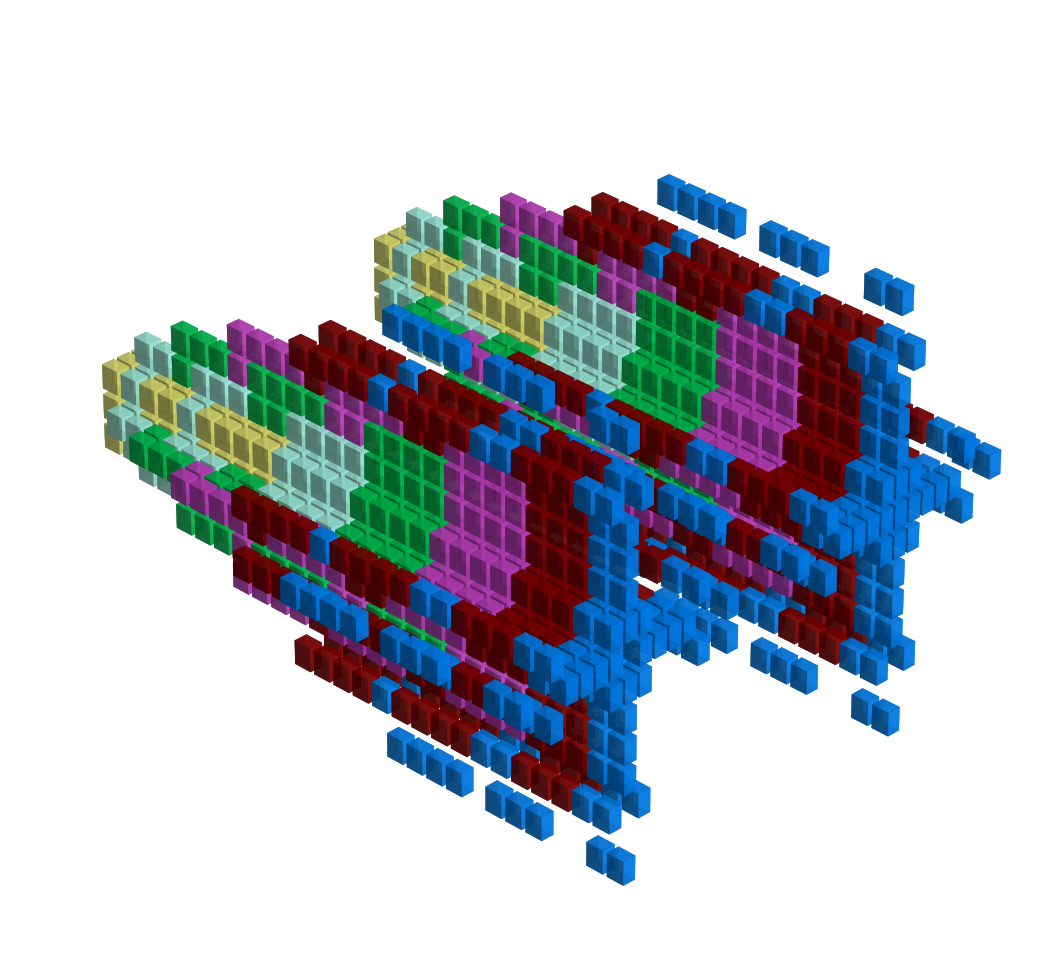
\includegraphics[width=14cm]{src/presets/pattern0-45.png}%           
  \end{adjustbox}                                                        
\caption{Evolution of Preset 0.}                                           
\end{figure}                                                               
\clearpage                                                                 
                                                                           
\begin{lstlisting}[basicstyle=\ttfamily\scriptsize,caption=Data structure for Preset 0.]
;preset0
  ; unusedPresetByte: Unused Byte
  .BYTE $00
  ; smoothingDelay: 'Because of the time taken to draw larger patterns speed
  ; increase/decrease is not linear. You can adjust the 'compensating delay'
  ; which often smooths out jerky patterns. Can be used just for special FX),
  ; though. Suck it and see.'
  .BYTE $0C
  ; cursorSpeed: 'Gives you a slow or fast little cursor, according to setting.'
  .BYTE $02
  ; bufferLength: 'Larger patterns flow more smoothly with a shorter
  ; Buffer Length - not so many positions are retained so less plotting to do.
  ; Small patterns with a long Buffer Length are good for 'steamer' effects.
  ; N.B. Cannot be adjusted whilst patterns are actually onscreen.'
  .BYTE $1F
  ; pulseSpeed: 'Usually if you hold down the button you get a continuous
  ; stream. Setting the Pulse Speed allows you to generate a pulsed stream, as
  ; if you were rapidly pressing and releasing the FIRE button.'
  .BYTE $01
  ; indexForColorBarDisplay: 'The initial index for the color displayed
  ; in the color bar when adjusting the colors for each step.'
  .BYTE $01
  ; lineWidth: 'Sets the width of the lines produced in Line Mode.'
  .BYTE $07
  ; sequencerSpeed: 'Controls the rate at which sequencer feeds in its data. '
  .BYTE $04
  ; pulseWidth: 'Sets the length of the pulses in a pulsed stream output.
  ; Don't worry about what that means - just get in there and mess with it.'
  .BYTE $01
  ; baseLevel: 'Controls how many 'levels' of pattern are plotted.'
  .BYTE $07
  ; presetColorValuesArray: 'Allows you to set the colour for each of the
  ; seven pattern steps. Set up the colour you want, press RETURN, and the
  ; command offers the next colour along, up to no. 7, then ends. Cannot be
  ; adjusted while patterns being generated.'
  .BYTE BLACK,BLUE,RED,PURPLE,GREEN,CYAN,YELLOW,WHITE
  ; trackingActivated: 'Controls whether logic-seeking is used in the
  ; buffer or not. The upshot of this for you is a slightly different feel -
  ; continuous but fragmented when ON, or together-ish bursts when OFF. Try it.'
  .BYTE $00
  ; lineModeActivated: 'A bit like drawing with the Aurora Borealis'
  .BYTE $00
  ; presetIndex: 'This calls in one of the 16 presets, stored Lightsynth
  ; parameters which give different effects. Try them all out io see some uf
  ; the multitude of effects which you cai achieve using the system. Some are
  ; fast, some slow, some pulse, others swirl. Play with them all, try them to
  ; different music.'
  .BYTE $00
  ; currentPatternElement: 'Initial pattern used by this preset.'
  .BYTE $00
  ; currentSymmetrySetting: 'Current symmetry setting.'
  ; Possible values are 0 - 4:
  ; 'NO SYMMETRY     '
  ; 'Y-AXIS SYMMETRY '
  ; 'X-Y SYMMETRY    '
  ; 'X-AXIS SYMMETRY '
  ; 'QUAD SYMMETRY   '
  .BYTE $01
  ; Unused Data.
  .BYTE $FF,$00,$FF,$FF,$00,$FF,$00,$FF,$00
\end{lstlisting}

\clearpage
\begin{lstlisting}
; This is where the presets get loaded to. It represents
; the data structure for the presets.
; currentVariableMode is an index into this data structure
; when the user adjusts settings.
presetValueArray
unusedPresetByte        .BYTE $00
smoothingDelay          .BYTE $0C
cursorSpeed             .BYTE $02
bufferLength            .BYTE $1F
pulseSpeed              .BYTE $01
indexForColorBarDisplay .BYTE $01
lineWidth               .BYTE $07
sequencerSpeed          .BYTE $04
pulseWidth              .BYTE $01
baseLevel               .BYTE $07
presetColorValuesArray  .BYTE BLACK,BLUE,RED,PURPLE,GREEN,CYAN,YELLOW,WHITE
trackingActivated       .BYTE $FF
lineModeActivated       .BYTE $00
patternIndex            .BYTE $05
\end{lstlisting}
\begin{lstlisting}
;-----------------------------------------------------
; LoadSelectedPresetSequence
;------------------------------------------------------
LoadSelectedPresetSequence    
        LDA #$FF
        STA currentModeActive

        ; Copy the value from the preset sequence into 
        ; current storage.
        LDY #COLOR_BAR_CURRENT
b16E1   LDA (presetSequenceDataLoPtr),Y
        STA presetValueArray,Y
        INY 
        CPY #$15
        BNE b16E1

        LDA (presetSequenceDataLoPtr),Y
        STA currentPatternElement
        INY 
        LDA (presetSequenceDataLoPtr),Y
        STA currentSymmetrySetting
        JMP WriteLastLineBufferAndReturn
        ; Returns
\end{lstlisting}
\clearpage

\textbf{Lines 1189-1231. \icode{\textbf{presetValueArray}}:} 
\textbf{Lines 1189-1231. \icode{\textbf{LoadSelectedPresetSequence}}:} 
\clearpage


\clearpage                                                                 
\begin{figure}[H]                                                          
  \centering                                                             
  \begin{adjustbox}{width=14cm,center}                                   
  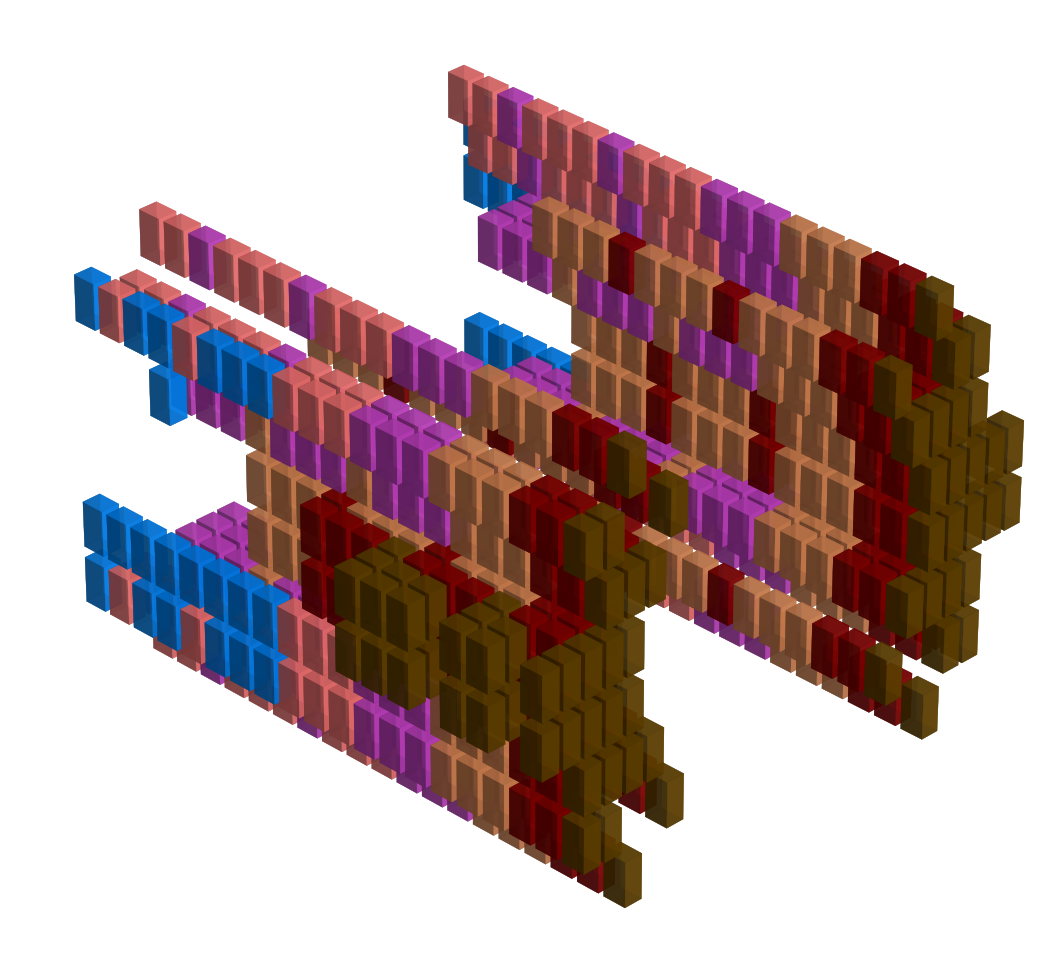
\includegraphics[width=14cm]{src/presets/pattern1-45.png}%           
  \end{adjustbox}                                                        
\caption{Evolution of Preset 1.}                                           
\end{figure}                                                               
\clearpage                                                                 
                                                                           
\begin{lstlisting}[basicstyle=\ttfamily\scriptsize,caption=Data structure for Preset 1.]
preset1
  ; unusedPresetByte: Unused Byte
  .BYTE $00
  ; smoothingDelay: 'Because of the time taken to draw larger patterns speed
  ; increase/decrease is not linear. You can adjust the 'compensating delay'
  ; which often smooths out jerky patterns. Can be used just for special FX),
  ; though. Suck it and see.'
  .BYTE $0C
  ; cursorSpeed: 'Gives you a slow or fast little cursor, according to setting.'
  .BYTE $02
  ; bufferLength: 'Larger patterns flow more smoothly with a shorter
  ; Buffer Length - not so many positions are retained so less plotting to do.
  ; Small patterns with a long Buffer Length are good for 'steamer' effects.
  ; N.B. Cannot be adjusted whilst patterns are actually onscreen.'
  .BYTE $28
  ; pulseSpeed: 'Usually if you hold down the button you get a continuous
  ; stream. Setting the Pulse Speed allows you to generate a pulsed stream, as
  ; if you were rapidly pressing and releasing the FIRE button.'
  .BYTE $01
  ; indexForColorBarDisplay: 'The initial index for the color displayed
  ; in the color bar when adjusting the colors for each step.'
  .BYTE $0E
  ; lineWidth: 'Sets the width of the lines produced in Line Mode.'
  .BYTE $07
  ; sequencerSpeed: 'Controls the rate at which sequencer feeds in its data. '
  .BYTE $08
  ; pulseWidth: 'Sets the length of the pulses in a pulsed stream output.
  ; Don't worry about what that means - just get in there and mess with it.'
  .BYTE $01
  ; baseLevel: 'Controls how many 'levels' of pattern are plotted.'
  .BYTE $07
  ; presetColorValuesArray: 'Allows you to set the colour for each of the
  ; seven pattern steps. Set up the colour you want, press RETURN, and the
  ; command offers the next colour along, up to no. 7, then ends. Cannot be
  ; adjusted while patterns being generated.'
  .BYTE BLACK,BROWN,RED,ORANGE,PURPLE,LTRED,BLUE,LTBLUE
  ; trackingActivated: 'Controls whether logic-seeking is used in the
  ; buffer or not. The upshot of this for you is a slightly different feel -
  ; continuous but fragmented when ON, or together-ish bursts when OFF. Try it.'
  .BYTE $FF
  ; lineModeActivated: 'A bit like drawing with the Aurora Borealis'
  .BYTE $00
  ; presetIndex: 'This calls in one of the 16 presets, stored Lightsynth
  ; parameters which give different effects. Try them all out io see some uf
  ; the multitude of effects which you cai achieve using the system. Some are
  ; fast, some slow, some pulse, others swirl. Play with them all, try them to
  ; different music.'
  .BYTE $01
  ; currentPatternElement: 'Initial pattern used by this preset.'
  .BYTE $01
  ; currentSymmetrySetting: 'Current symmetry setting.'
  ; Possible values are 0 - 4:
  ; 'NO SYMMETRY     '
  ; 'Y-AXIS SYMMETRY '
  ; 'X-Y SYMMETRY    '
  ; 'X-AXIS SYMMETRY '
  ; 'QUAD SYMMETRY   '
  .BYTE $04
  ; Unused Data.
  .BYTE $FF,$00,$FF,$FF,$00,$FF,$00,$FF,$00
\end{lstlisting}

\clearpage
\begin{lstlisting}
presetKeyCodes
        .BYTE KEY_LEFT,KEY_1,KEY_2,KEY_3,KEY_4,KEY_5,KEY_6,KEY_7
        .BYTE KEY_8,KEY_9,KEY_0,KEY_PLUS,KEY_MINUS,KEY_POUND
        .BYTE KEY_CLR_HOME,KEY_INST_DEL
\end{lstlisting}
\begin{lstlisting}
;-------------------------------------------------------
; CheckKeyboardInput
;-------------------------------------------------------
CheckKeyboardInput   
        ...
        ; Check if one of the presets has been selected.
CheckIfPresetKeysPressed   
        LDX #$00
presetKeyLoop   
        CMP presetKeyCodes,X
        BEQ UpdateDisplayedPreset
        INX 
        CPX #$10
        BNE presetKeyLoop

        JMP MaybeWPressed

UpdateDisplayedPreset   
        JMP DisplayPresetMessage
\end{lstlisting}

\clearpage

\textbf{Lines 1189-1231. \icode{\textbf{CheckIfPresetKeysPressed}}:} 
\clearpage


\clearpage                                                                 
\begin{figure}[H]                                                          
  \centering                                                             
  \begin{adjustbox}{width=14cm,center}                                   
  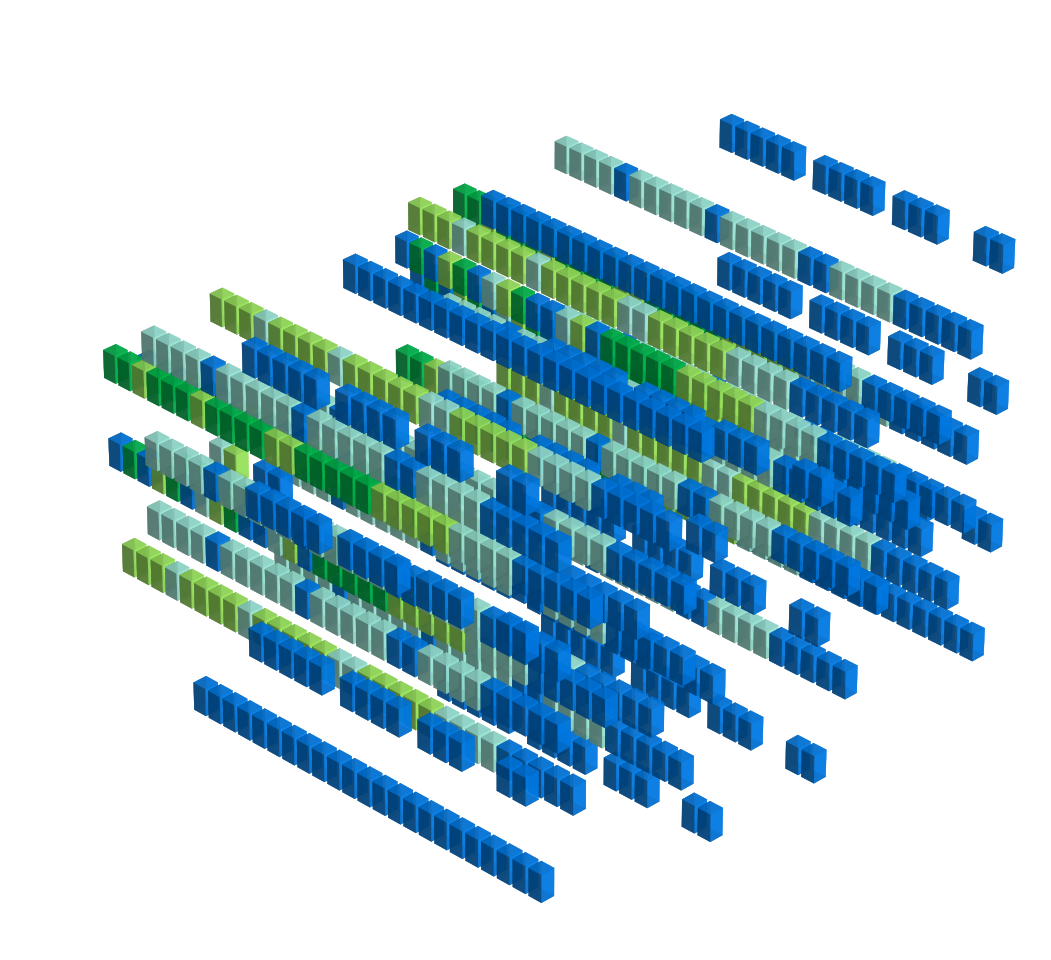
\includegraphics[width=14cm]{src/presets/pattern2-45.png}%           
  \end{adjustbox}                                                        
\caption{Evolution of Preset 2.}                                           
\end{figure}                                                               
\clearpage                                                                 
                                                                           
\begin{lstlisting}[basicstyle=\ttfamily\scriptsize,caption=Data structure for Preset 2.]
preset2
  ; unusedPresetByte: Unused Byte
  .BYTE $00
  ; smoothingDelay: 'Because of the time taken to draw larger patterns speed
  ; increase/decrease is not linear. You can adjust the 'compensating delay'
  ; which often smooths out jerky patterns. Can be used just for special FX),
  ; though. Suck it and see.'
  .BYTE $0B
  ; cursorSpeed: 'Gives you a slow or fast little cursor, according to setting.'
  .BYTE $02
  ; bufferLength: 'Larger patterns flow more smoothly with a shorter
  ; Buffer Length - not so many positions are retained so less plotting to do.
  ; Small patterns with a long Buffer Length are good for 'steamer' effects.
  ; N.B. Cannot be adjusted whilst patterns are actually onscreen.'
  .BYTE $28
  ; pulseSpeed: 'Usually if you hold down the button you get a continuous
  ; stream. Setting the Pulse Speed allows you to generate a pulsed stream, as
  ; if you were rapidly pressing and releasing the FIRE button.'
  .BYTE $01
  ; indexForColorBarDisplay: 'The initial index for the color displayed
  ; in the color bar when adjusting the colors for each step.'
  .BYTE $01
  ; lineWidth: 'Sets the width of the lines produced in Line Mode.'
  .BYTE $07
  ; sequencerSpeed: 'Controls the rate at which sequencer feeds in its data. '
  .BYTE $0B
  ; pulseWidth: 'Sets the length of the pulses in a pulsed stream output.
  ; Don't worry about what that means - just get in there and mess with it.'
  .BYTE $01
  ; baseLevel: 'Controls how many 'levels' of pattern are plotted.'
  .BYTE $07
  ; presetColorValuesArray: 'Allows you to set the colour for each of the
  ; seven pattern steps. Set up the colour you want, press RETURN, and the
  ; command offers the next colour along, up to no. 7, then ends. Cannot be
  ; adjusted while patterns being generated.'
  .BYTE BLACK,BLUE,LTBLUE,CYAN,LTGREEN,GREEN,LTBLUE,BLUE
  ; trackingActivated: 'Controls whether logic-seeking is used in the
  ; buffer or not. The upshot of this for you is a slightly different feel -
  ; continuous but fragmented when ON, or together-ish bursts when OFF. Try it.'
  .BYTE $FF
  ; lineModeActivated: 'A bit like drawing with the Aurora Borealis'
  .BYTE $00
  ; presetIndex: 'This calls in one of the 16 presets, stored Lightsynth
  ; parameters which give different effects. Try them all out io see some uf
  ; the multitude of effects which you cai achieve using the system. Some are
  ; fast, some slow, some pulse, others swirl. Play with them all, try them to
  ; different music.'
  .BYTE $05
  ; currentPatternElement: 'Initial pattern used by this preset.'
  .BYTE $05
  ; currentSymmetrySetting: 'Current symmetry setting.'
  ; Possible values are 0 - 4:
  ; 'NO SYMMETRY     '
  ; 'Y-AXIS SYMMETRY '
  ; 'X-Y SYMMETRY    '
  ; 'X-AXIS SYMMETRY '
  ; 'QUAD SYMMETRY   '
  .BYTE $01
  ; Unused Data.
  .BYTE $FF,$00,$FF,$FF,$00,$FF,$00,$FF,$00
\end{lstlisting}

\clearpage
\begin{lstlisting}
;-------------------------------------------------------
; DisplayPresetMessage
;-------------------------------------------------------
DisplayPresetMessage    
        LDA shiftPressed
        AND #$04
        BEQ SelectNewPreset
        JMP EditCustomPattern

SelectNewPreset
        TXA 
        PHA 
        JSR ClearLastLineOfScreen
        LDX #$00
b1613   LDA txtPreset,X
        STA lastLineBufferPtr,X
        INX 
        CPX #$10
        BNE b1613

        PLA 
        PHA 
        TAX 
        BEQ b1638
b1623   INC dataFreeDigitThree
        LDA dataFreeDigitThree
        CMP #$BA
        BNE b1635
        LDA #$30
        STA dataFreeDigitThree
        INC dataFreeDigitTwo
b1635   DEX 
        BNE b1623

b1638   JMP UpdateCurrentActivePreset

WriteLastLineBufferAndReturn    
        JSR WriteLastLineBufferToScreen
        RTS 

.enc "petscii" 
txtPreset
        .TEXT 'PRESET ',$B0,$B0,'      ',$BA
txtPresetActivatedStored
        .TEXT ' ACTIVATED       '
        .TEXT 'DATA STORED    '
.enc "none" 
\end{lstlisting}
\clearpage

\textbf{Lines 1189-1231. \icode{\textbf{DisplayPresetMessage}}:} 
\clearpage

\begin{figure}[H]                                                          
  \centering                                                             
  \begin{adjustbox}{width=14cm,center}                                   
  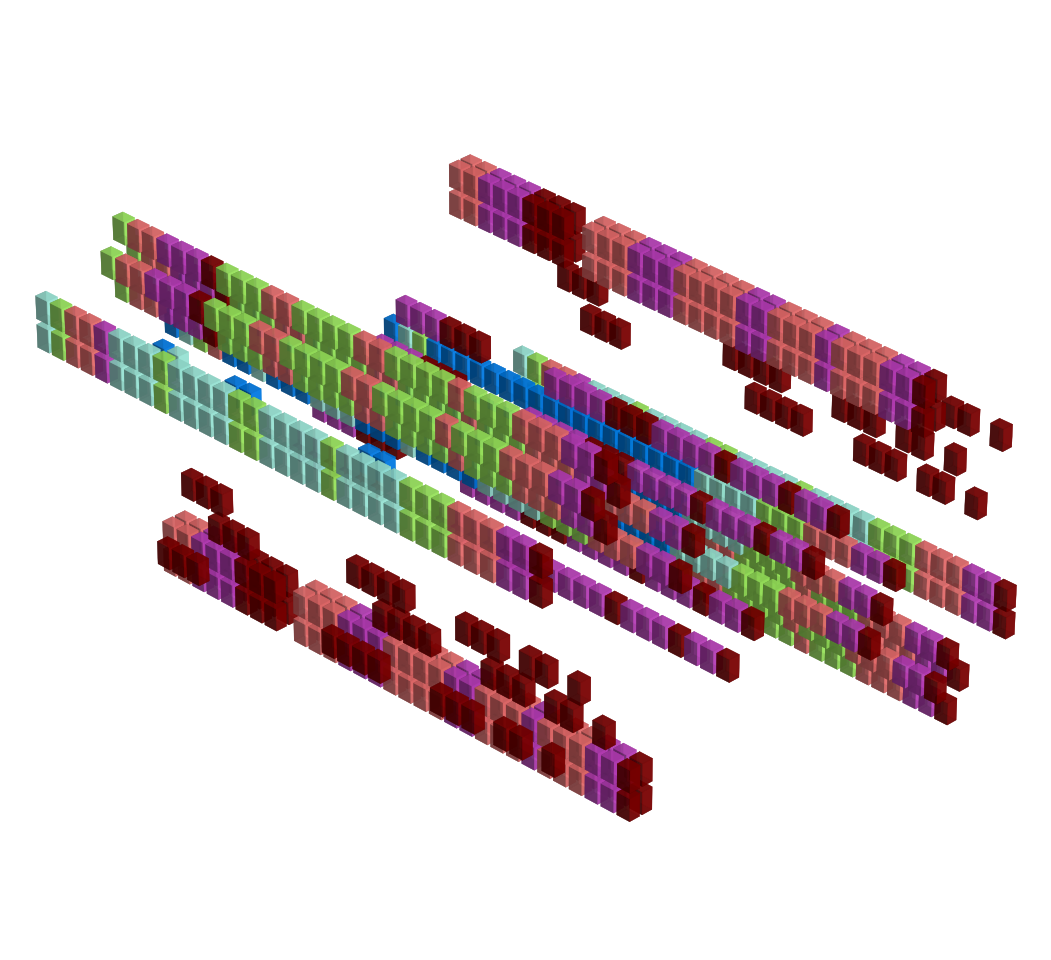
\includegraphics[width=14cm]{src/presets/pattern3-45.png}%           
  \end{adjustbox}                                                        
\caption{Evolution of Preset 3.}                                           
\end{figure}                                                               
\clearpage                                                                 
                                                                           
\begin{lstlisting}[basicstyle=\ttfamily\scriptsize,caption=Data structure for Preset 3.]
preset3
  ; unusedPresetByte: Unused Byte
  .BYTE $00
  ; smoothingDelay: 'Because of the time taken to draw larger patterns speed
  ; increase/decrease is not linear. You can adjust the 'compensating delay'
  ; which often smooths out jerky patterns. Can be used just for special FX),
  ; though. Suck it and see.'
  .BYTE $04
  ; cursorSpeed: 'Gives you a slow or fast little cursor, according to setting.'
  .BYTE $02
  ; bufferLength: 'Larger patterns flow more smoothly with a shorter
  ; Buffer Length - not so many positions are retained so less plotting to do.
  ; Small patterns with a long Buffer Length are good for 'steamer' effects.
  ; N.B. Cannot be adjusted whilst patterns are actually onscreen.'
  .BYTE $26
  ; pulseSpeed: 'Usually if you hold down the button you get a continuous
  ; stream. Setting the Pulse Speed allows you to generate a pulsed stream, as
  ; if you were rapidly pressing and releasing the FIRE button.'
  .BYTE $01
  ; indexForColorBarDisplay: 'The initial index for the color displayed
  ; in the color bar when adjusting the colors for each step.'
  .BYTE $01
  ; lineWidth: 'Sets the width of the lines produced in Line Mode.'
  .BYTE $07
  ; sequencerSpeed: 'Controls the rate at which sequencer feeds in its data. '
  .BYTE $0A
  ; pulseWidth: 'Sets the length of the pulses in a pulsed stream output.
  ; Don't worry about what that means - just get in there and mess with it.'
  .BYTE $01
  ; baseLevel: 'Controls how many 'levels' of pattern are plotted.'
  .BYTE $07
  ; presetColorValuesArray: 'Allows you to set the colour for each of the
  ; seven pattern steps. Set up the colour you want, press RETURN, and the
  ; command offers the next colour along, up to no. 7, then ends. Cannot be
  ; adjusted while patterns being generated.'
  .BYTE BLACK,RED,PURPLE,LTRED,LTGREEN,CYAN,LTBLUE,BLUE
  ; trackingActivated: 'Controls whether logic-seeking is used in the
  ; buffer or not. The upshot of this for you is a slightly different feel -
  ; continuous but fragmented when ON, or together-ish bursts when OFF. Try it.'
  .BYTE $00
  ; lineModeActivated: 'A bit like drawing with the Aurora Borealis'
  .BYTE $00
  ; presetIndex: 'This calls in one of the 16 presets, stored Lightsynth
  ; parameters which give different effects. Try them all out io see some uf
  ; the multitude of effects which you cai achieve using the system. Some are
  ; fast, some slow, some pulse, others swirl. Play with them all, try them to
  ; different music.'
  .BYTE $0E
  ; currentPatternElement: 'Initial pattern used by this preset.'
  .BYTE $0E
  ; currentSymmetrySetting: 'Current symmetry setting.'
  ; Possible values are 0 - 4:
  ; 'NO SYMMETRY     '
  ; 'Y-AXIS SYMMETRY '
  ; 'X-Y SYMMETRY    '
  ; 'X-AXIS SYMMETRY '
  ; 'QUAD SYMMETRY   '
  .BYTE $02
  ; Unused Data.
  .BYTE $FF,$00,$FF,$FF,$00,$FF,$00,$EA,$10
\end{lstlisting}

\clearpage
\begin{lstlisting}
;-------------------------------------------------------
; UpdateCurrentActivePreset
;-------------------------------------------------------
UpdateCurrentActivePreset    
        LDA shiftPressed
        AND #$01
        ASL 
        ASL 
        ASL 
        ASL 
        TAY 

        LDX #$00
b167C   LDA txtPresetActivatedStored,Y
        STA customPatternValueBufferMessage,X
        INY 
        INX 
        CPX #$10
        BNE b167C

        LDA shiftPressed
        AND #$01
        BNE b1692
        JMP RefreshPresetData

b1692   PLA 
        TAX 
        JSR GetPresetPointersUsingXRegister

        LDY #$00
        LDX #$00
b169B   LDA presetValueArray,X
        STA (presetSequenceDataLoPtr),Y
        INY 
        INX 
        CPX #$15
        BNE b169B

        LDA currentPatternElement
        STA (presetSequenceDataLoPtr),Y
        INY 
        LDA currentSymmetrySetting
        STA (presetSequenceDataLoPtr),Y
        JMP WriteLastLineBufferAndReturn
\end{lstlisting}
\clearpage

\textbf{Lines 1189-1231. \icode{\textbf{UpdateCurrentActivePreset}}:} 
\clearpage

\clearpage                                                                 
\begin{figure}[H]                                                          
  \centering                                                             
  \begin{adjustbox}{width=14cm,center}                                   
  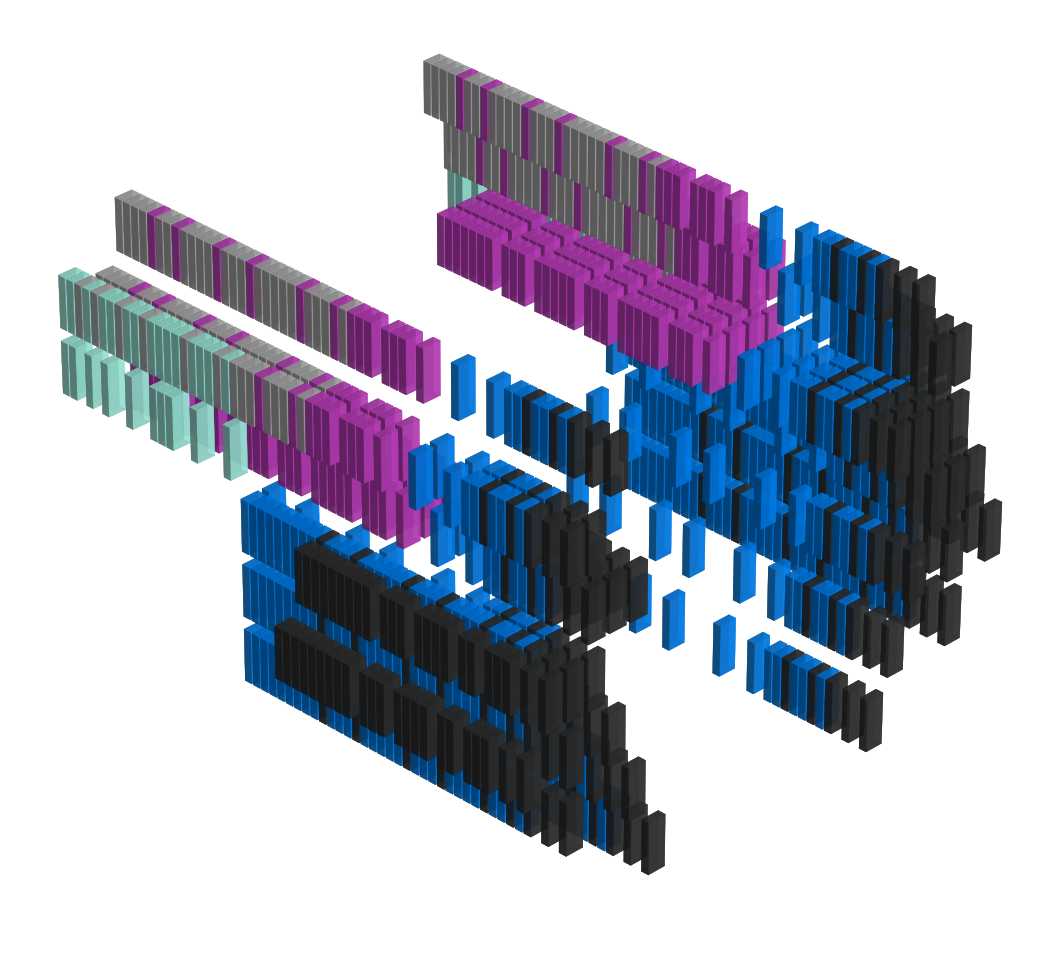
\includegraphics[width=14cm]{src/presets/pattern4-45.png}%           
  \end{adjustbox}                                                        
\caption{Evolution of Preset 4.}                                           
\end{figure}                                                               
\clearpage                                                                 
                                                                           
\begin{lstlisting}[basicstyle=\ttfamily\scriptsize,caption=Data structure for Preset 4.]
preset4
  ; unusedPresetByte: Unused Byte
  .BYTE $00
  ; smoothingDelay: 'Because of the time taken to draw larger patterns speed
  ; increase/decrease is not linear. You can adjust the 'compensating delay'
  ; which often smooths out jerky patterns. Can be used just for special FX),
  ; though. Suck it and see.'
  .BYTE $0C
  ; cursorSpeed: 'Gives you a slow or fast little cursor, according to setting.'
  .BYTE $01
  ; bufferLength: 'Larger patterns flow more smoothly with a shorter
  ; Buffer Length - not so many positions are retained so less plotting to do.
  ; Small patterns with a long Buffer Length are good for 'steamer' effects.
  ; N.B. Cannot be adjusted whilst patterns are actually onscreen.'
  .BYTE $2B
  ; pulseSpeed: 'Usually if you hold down the button you get a continuous
  ; stream. Setting the Pulse Speed allows you to generate a pulsed stream, as
  ; if you were rapidly pressing and releasing the FIRE button.'
  .BYTE $01
  ; indexForColorBarDisplay: 'The initial index for the color displayed
  ; in the color bar when adjusting the colors for each step.'
  .BYTE $07
  ; lineWidth: 'Sets the width of the lines produced in Line Mode.'
  .BYTE $07
  ; sequencerSpeed: 'Controls the rate at which sequencer feeds in its data. '
  .BYTE $08
  ; pulseWidth: 'Sets the length of the pulses in a pulsed stream output.
  ; Don't worry about what that means - just get in there and mess with it.'
  .BYTE $01
  ; baseLevel: 'Controls how many 'levels' of pattern are plotted.'
  .BYTE $07
  ; presetColorValuesArray: 'Allows you to set the colour for each of the
  ; seven pattern steps. Set up the colour you want, press RETURN, and the
  ; command offers the next colour along, up to no. 7, then ends. Cannot be
  ; adjusted while patterns being generated.'
  .BYTE BLACK,GRAY1,BLUE,GRAY2,PURPLE,GRAY3,CYAN,WHITE
  ; trackingActivated: 'Controls whether logic-seeking is used in the
  ; buffer or not. The upshot of this for you is a slightly different feel -
  ; continuous but fragmented when ON, or together-ish bursts when OFF. Try it.'
  .BYTE $00
  ; lineModeActivated: 'A bit like drawing with the Aurora Borealis'
  .BYTE $00
  ; presetIndex: 'This calls in one of the 16 presets, stored Lightsynth
  ; parameters which give different effects. Try them all out io see some uf
  ; the multitude of effects which you cai achieve using the system. Some are
  ; fast, some slow, some pulse, others swirl. Play with them all, try them to
  ; different music.'
  .BYTE $01
  ; currentPatternElement: 'Initial pattern used by this preset.'
  .BYTE $01
  ; currentSymmetrySetting: 'Current symmetry setting.'
  ; Possible values are 0 - 4:
  ; 'NO SYMMETRY     '
  ; 'Y-AXIS SYMMETRY '
  ; 'X-Y SYMMETRY    '
  ; 'X-AXIS SYMMETRY '
  ; 'QUAD SYMMETRY   '
  .BYTE $01
  ; Unused Data.
  .BYTE $00,$FF,$00,$00,$FF,$00,$FF,$00,$FF
\end{lstlisting}

\clearpage
\begin{lstlisting}[basicstyle=\ttfamily\scriptsize]
;--------------------------------------------
; RefreshPresetData
;--------------------------------------------
RefreshPresetData    
        PLA 
        TAX 
        JSR GetPresetPointersUsingXRegister
        LDY #BUFFER_LENGTH
        LDA (presetSequenceDataLoPtr),Y
        CMP bufferLength
        BEQ b16C6

        JSR ResetCurrentActiveMode
        JMP LoadSelectedPresetSequence
        ; Returns

        ; Check the preset against current data
        ; and reload if different.
b16C6   LDX #$00
        LDY #SEQUENCER_SPEED
b16CA   LDA (presetSequenceDataLoPtr),Y
        CMP presetColorValuesArray,X
        BNE LoadSelectedPresetSequence
        INY 
        INX 
        CPX #$08
        BNE b16CA

        JMP LoadSelectedPresetSequence

;---------------------------------------------
; GetPresetPointersUsingXRegister
;---------------------------------------------
GetPresetPointersUsingXRegister   
        LDA #>presetSequenceData
        STA presetSequenceDataHiPtr
        LDA #<presetSequenceData
        STA presetSequenceDataLoPtr
        TXA 
        BEQ b1712

        ; Skip through the preset data until we get to the position
        ; storing the preset data for the sequence indicated by the X
        ; register.
b1702   LDA presetSequenceDataLoPtr
        CLC 
        ADC #$20
        STA presetSequenceDataLoPtr
        LDA presetSequenceDataHiPtr
        ADC #$00
        STA presetSequenceDataHiPtr
        DEX 
        BNE b1702
b1712   RTS 

\end{lstlisting}
\clearpage

\textbf{Lines 1189-1231. \icode{\textbf{DisplayPresetMessage}}:} 
\clearpage

\clearpage                                                                 
\begin{figure}[H]                                                          
  \centering                                                             
  \begin{adjustbox}{width=14cm,center}                                   
  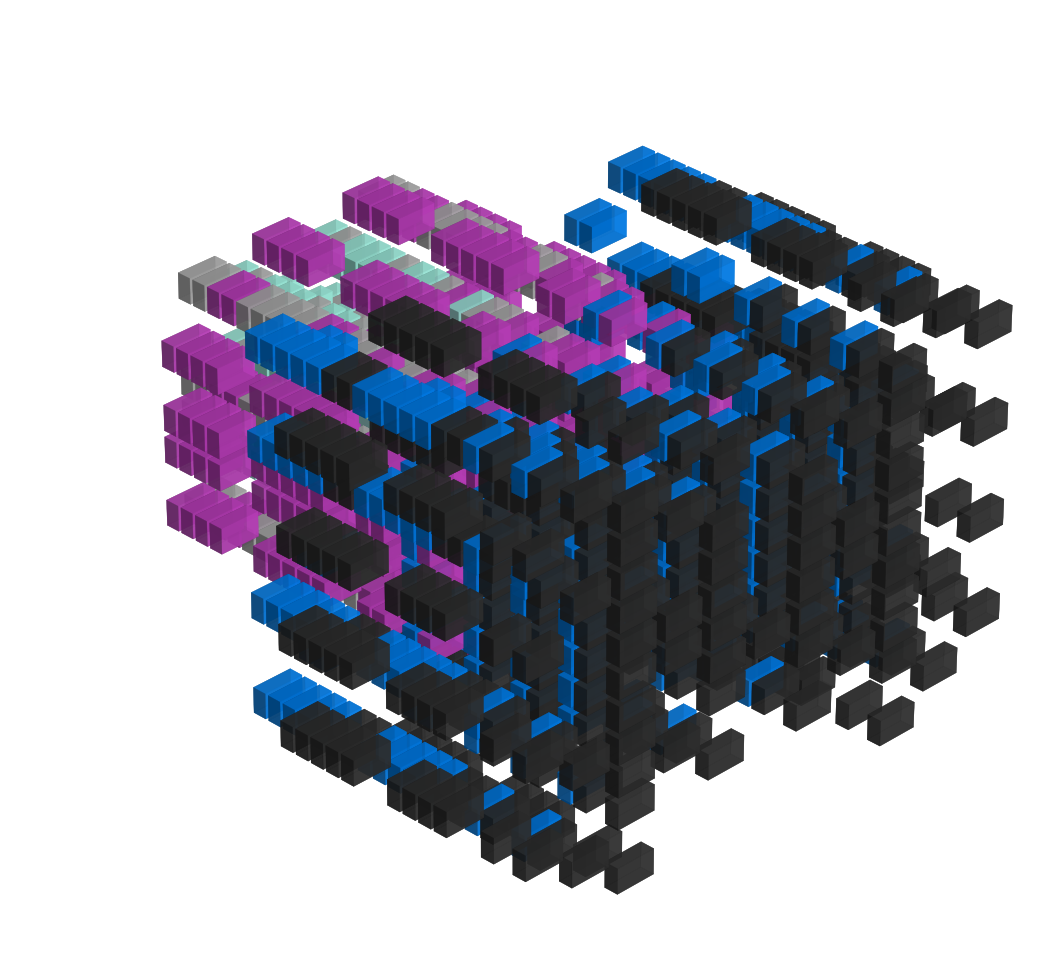
\includegraphics[width=14cm]{src/presets/pattern5-45.png}%           
  \end{adjustbox}                                                        
\caption{Evolution of Preset 5.}                                           
\end{figure}                                                               
\clearpage                                                                 
                                                                           
\begin{lstlisting}[basicstyle=\ttfamily\scriptsize,caption=Data structure for Preset 5.]
preset5
  ; unusedPresetByte: Unused Byte
  .BYTE $00
  ; smoothingDelay: 'Because of the time taken to draw larger patterns speed
  ; increase/decrease is not linear. You can adjust the 'compensating delay'
  ; which often smooths out jerky patterns. Can be used just for special FX),
  ; though. Suck it and see.'
  .BYTE $0C
  ; cursorSpeed: 'Gives you a slow or fast little cursor, according to setting.'
  .BYTE $02
  ; bufferLength: 'Larger patterns flow more smoothly with a shorter
  ; Buffer Length - not so many positions are retained so less plotting to do.
  ; Small patterns with a long Buffer Length are good for 'steamer' effects.
  ; N.B. Cannot be adjusted whilst patterns are actually onscreen.'
  .BYTE $2B
  ; pulseSpeed: 'Usually if you hold down the button you get a continuous
  ; stream. Setting the Pulse Speed allows you to generate a pulsed stream, as
  ; if you were rapidly pressing and releasing the FIRE button.'
  .BYTE $01
  ; indexForColorBarDisplay: 'The initial index for the color displayed
  ; in the color bar when adjusting the colors for each step.'
  .BYTE $07
  ; lineWidth: 'Sets the width of the lines produced in Line Mode.'
  .BYTE $07
  ; sequencerSpeed: 'Controls the rate at which sequencer feeds in its data. '
  .BYTE $0C
  ; pulseWidth: 'Sets the length of the pulses in a pulsed stream output.
  ; Don't worry about what that means - just get in there and mess with it.'
  .BYTE $01
  ; baseLevel: 'Controls how many 'levels' of pattern are plotted.'
  .BYTE $07
  ; presetColorValuesArray: 'Allows you to set the colour for each of the
  ; seven pattern steps. Set up the colour you want, press RETURN, and the
  ; command offers the next colour along, up to no. 7, then ends. Cannot be
  ; adjusted while patterns being generated.'
  .BYTE BLACK,GRAY1,BLUE,GRAY2,PURPLE,GRAY3,CYAN,WHITE
  ; trackingActivated: 'Controls whether logic-seeking is used in the
  ; buffer or not. The upshot of this for you is a slightly different feel -
  ; continuous but fragmented when ON, or together-ish bursts when OFF. Try it.'
  .BYTE $00
  ; lineModeActivated: 'A bit like drawing with the Aurora Borealis'
  .BYTE $00
  ; presetIndex: 'This calls in one of the 16 presets, stored Lightsynth
  ; parameters which give different effects. Try them all out io see some uf
  ; the multitude of effects which you cai achieve using the system. Some are
  ; fast, some slow, some pulse, others swirl. Play with them all, try them to
  ; different music.'
  .BYTE $06
  ; currentPatternElement: 'Initial pattern used by this preset.'
  .BYTE $06
  ; currentSymmetrySetting: 'Current symmetry setting.'
  ; Possible values are 0 - 4:
  ; 'NO SYMMETRY     '
  ; 'Y-AXIS SYMMETRY '
  ; 'X-Y SYMMETRY    '
  ; 'X-AXIS SYMMETRY '
  ; 'QUAD SYMMETRY   '
  .BYTE $03
  ; Unused Data.
  .BYTE $00,$FF,$00,$00,$FF,$00,$FF,$00,$F7
\end{lstlisting}


\clearpage                                                                 
\begin{figure}[H]                                                          
  \centering                                                             
  \begin{adjustbox}{width=14cm,center}                                   
  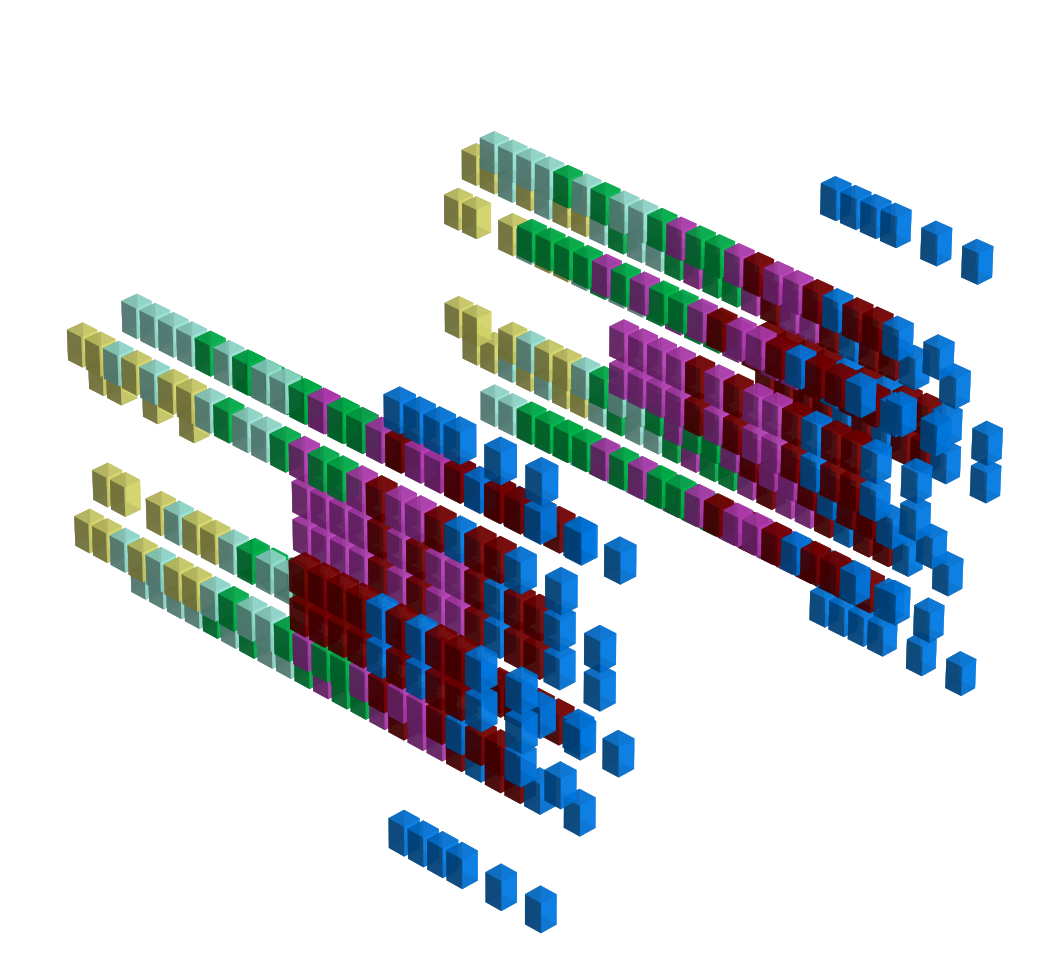
\includegraphics[width=14cm]{src/presets/pattern6-45.png}%           
  \end{adjustbox}                                                        
\caption{Evolution of Preset 6.}                                           
\end{figure}                                                               
\clearpage                                                                 
                                                                           
\begin{lstlisting}[basicstyle=\ttfamily\scriptsize,caption=Data structure for Preset 6.]
preset6
  ; unusedPresetByte: Unused Byte
  .BYTE $00
  ; smoothingDelay: 'Because of the time taken to draw larger patterns speed
  ; increase/decrease is not linear. You can adjust the 'compensating delay'
  ; which often smooths out jerky patterns. Can be used just for special FX),
  ; though. Suck it and see.'
  .BYTE $0F
  ; cursorSpeed: 'Gives you a slow or fast little cursor, according to setting.'
  .BYTE $02
  ; bufferLength: 'Larger patterns flow more smoothly with a shorter
  ; Buffer Length - not so many positions are retained so less plotting to do.
  ; Small patterns with a long Buffer Length are good for 'steamer' effects.
  ; N.B. Cannot be adjusted whilst patterns are actually onscreen.'
  .BYTE $3F
  ; pulseSpeed: 'Usually if you hold down the button you get a continuous
  ; stream. Setting the Pulse Speed allows you to generate a pulsed stream, as
  ; if you were rapidly pressing and releasing the FIRE button.'
  .BYTE $01
  ; indexForColorBarDisplay: 'The initial index for the color displayed
  ; in the color bar when adjusting the colors for each step.'
  .BYTE $01
  ; lineWidth: 'Sets the width of the lines produced in Line Mode.'
  .BYTE $07
  ; sequencerSpeed: 'Controls the rate at which sequencer feeds in its data. '
  .BYTE $0F
  ; pulseWidth: 'Sets the length of the pulses in a pulsed stream output.
  ; Don't worry about what that means - just get in there and mess with it.'
  .BYTE $01
  ; baseLevel: 'Controls how many 'levels' of pattern are plotted.'
  .BYTE $07
  ; presetColorValuesArray: 'Allows you to set the colour for each of the
  ; seven pattern steps. Set up the colour you want, press RETURN, and the
  ; command offers the next colour along, up to no. 7, then ends. Cannot be
  ; adjusted while patterns being generated.'
  .BYTE BLACK,BLUE,RED,PURPLE,GREEN,CYAN,YELLOW,WHITE
  ; trackingActivated: 'Controls whether logic-seeking is used in the
  ; buffer or not. The upshot of this for you is a slightly different feel -
  ; continuous but fragmented when ON, or together-ish bursts when OFF. Try it.'
  .BYTE $FF
  ; lineModeActivated: 'A bit like drawing with the Aurora Borealis'
  .BYTE $00
  ; presetIndex: 'This calls in one of the 16 presets, stored Lightsynth
  ; parameters which give different effects. Try them all out io see some uf
  ; the multitude of effects which you cai achieve using the system. Some are
  ; fast, some slow, some pulse, others swirl. Play with them all, try them to
  ; different music.'
  .BYTE $03
  ; currentPatternElement: 'Initial pattern used by this preset.'
  .BYTE $03
  ; currentSymmetrySetting: 'Current symmetry setting.'
  ; Possible values are 0 - 4:
  ; 'NO SYMMETRY     '
  ; 'Y-AXIS SYMMETRY '
  ; 'X-Y SYMMETRY    '
  ; 'X-AXIS SYMMETRY '
  ; 'QUAD SYMMETRY   '
  .BYTE $04
  ; Unused Data.
  .BYTE $00,$FF,$00,$00,$FF,$00,$FF,$00,$FF
\end{lstlisting}


\clearpage                                                                 
\begin{figure}[H]                                                          
  \centering                                                             
  \begin{adjustbox}{width=14cm,center}                                   
  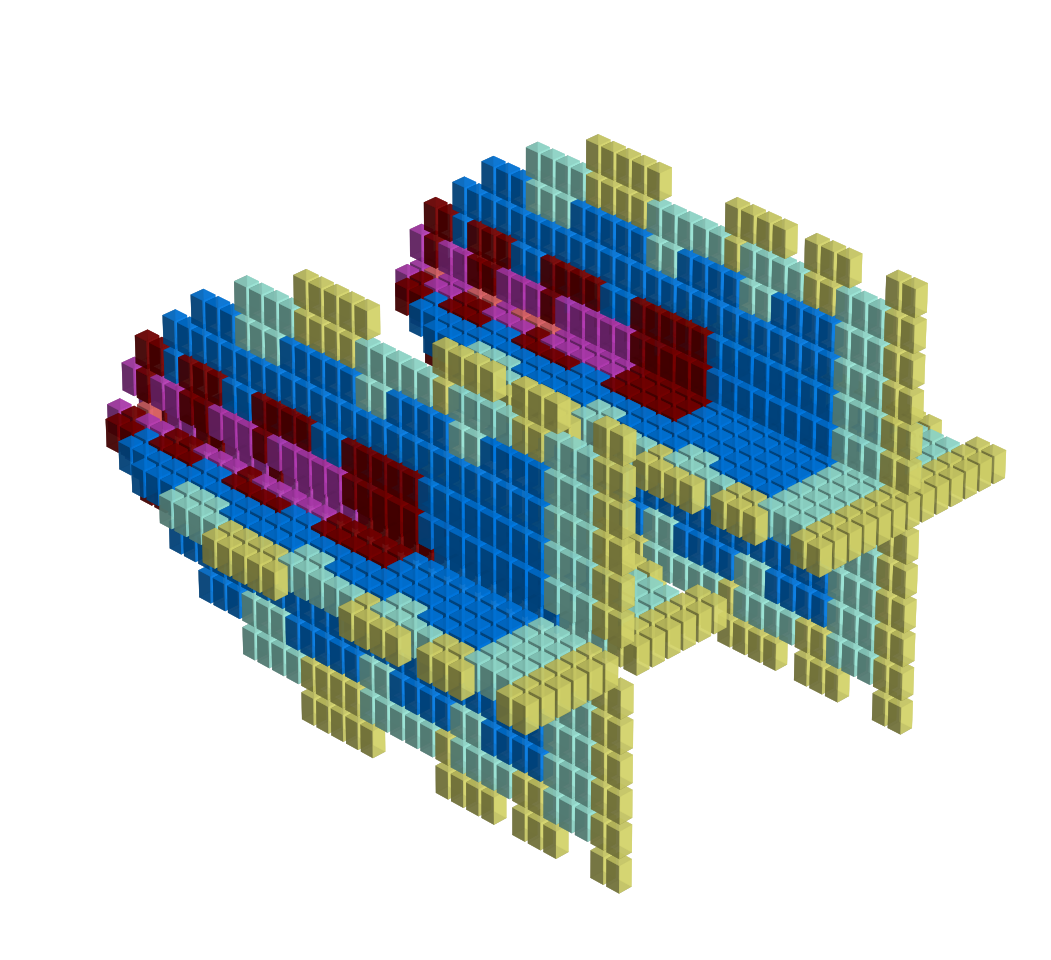
\includegraphics[width=14cm]{src/presets/pattern7-45.png}%           
  \end{adjustbox}                                                        
\caption{Evolution of Preset 7.}                                           
\end{figure}                                                               
\clearpage                                                                 
                                                                           
\begin{lstlisting}[basicstyle=\ttfamily\scriptsize,caption=Data structure for Preset 7.]
preset7
  ; unusedPresetByte: Unused Byte
  .BYTE $00
  ; smoothingDelay: 'Because of the time taken to draw larger patterns speed
  ; increase/decrease is not linear. You can adjust the 'compensating delay'
  ; which often smooths out jerky patterns. Can be used just for special FX),
  ; though. Suck it and see.'
  .BYTE $0B
  ; cursorSpeed: 'Gives you a slow or fast little cursor, according to setting.'
  .BYTE $01
  ; bufferLength: 'Larger patterns flow more smoothly with a shorter
  ; Buffer Length - not so many positions are retained so less plotting to do.
  ; Small patterns with a long Buffer Length are good for 'steamer' effects.
  ; N.B. Cannot be adjusted whilst patterns are actually onscreen.'
  .BYTE $1C
  ; pulseSpeed: 'Usually if you hold down the button you get a continuous
  ; stream. Setting the Pulse Speed allows you to generate a pulsed stream, as
  ; if you were rapidly pressing and releasing the FIRE button.'
  .BYTE $02
  ; indexForColorBarDisplay: 'The initial index for the color displayed
  ; in the color bar when adjusting the colors for each step.'
  .BYTE $0A
  ; lineWidth: 'Sets the width of the lines produced in Line Mode.'
  .BYTE $07
  ; sequencerSpeed: 'Controls the rate at which sequencer feeds in its data. '
  .BYTE $09
  ; pulseWidth: 'Sets the length of the pulses in a pulsed stream output.
  ; Don't worry about what that means - just get in there and mess with it.'
  .BYTE $01
  ; baseLevel: 'Controls how many 'levels' of pattern are plotted.'
  .BYTE $07
  ; presetColorValuesArray: 'Allows you to set the colour for each of the
  ; seven pattern steps. Set up the colour you want, press RETURN, and the
  ; command offers the next colour along, up to no. 7, then ends. Cannot be
  ; adjusted while patterns being generated.'
  .BYTE BLACK,YELLOW,CYAN,LTBLUE,BLUE,RED,PURPLE,LTRED
  ; trackingActivated: 'Controls whether logic-seeking is used in the
  ; buffer or not. The upshot of this for you is a slightly different feel -
  ; continuous but fragmented when ON, or together-ish bursts when OFF. Try it.'
  .BYTE $00
  ; lineModeActivated: 'A bit like drawing with the Aurora Borealis'
  .BYTE $00
  ; presetIndex: 'This calls in one of the 16 presets, stored Lightsynth
  ; parameters which give different effects. Try them all out io see some uf
  ; the multitude of effects which you cai achieve using the system. Some are
  ; fast, some slow, some pulse, others swirl. Play with them all, try them to
  ; different music.'
  .BYTE $07
  ; currentPatternElement: 'Initial pattern used by this preset.'
  .BYTE $07
  ; currentSymmetrySetting: 'Current symmetry setting.'
  ; Possible values are 0 - 4:
  ; 'NO SYMMETRY     '
  ; 'Y-AXIS SYMMETRY '
  ; 'X-Y SYMMETRY    '
  ; 'X-AXIS SYMMETRY '
  ; 'QUAD SYMMETRY   '
  .BYTE $01
  ; Unused Data.
  .BYTE $00,$FF,$00,$00,$FF,$00,$FF,$15,$EF
\end{lstlisting}


\clearpage                                                                 
\begin{figure}[H]                                                          
  \centering                                                             
  \begin{adjustbox}{width=14cm,center}                                   
  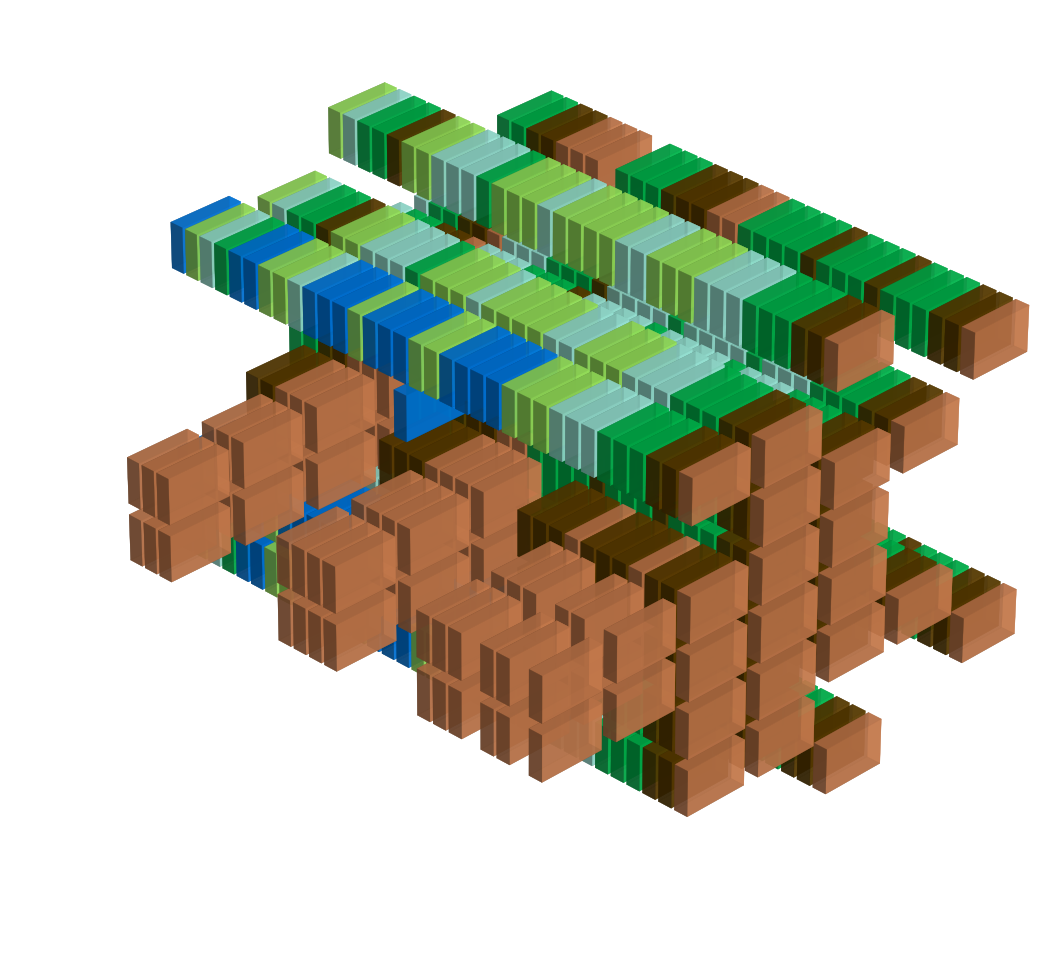
\includegraphics[width=14cm]{src/presets/pattern8-45.png}%           
  \end{adjustbox}                                                        
\caption{Evolution of Preset 8.}                                           
\end{figure}                                                               
\clearpage                                                                 
                                                                           
\begin{lstlisting}[basicstyle=\ttfamily\scriptsize,caption=Data structure for Preset 8.]
preset8
  ; unusedPresetByte: Unused Byte
  .BYTE $00
  ; smoothingDelay: 'Because of the time taken to draw larger patterns speed
  ; increase/decrease is not linear. You can adjust the 'compensating delay'
  ; which often smooths out jerky patterns. Can be used just for special FX),
  ; though. Suck it and see.'
  .BYTE $04
  ; cursorSpeed: 'Gives you a slow or fast little cursor, according to setting.'
  .BYTE $01
  ; bufferLength: 'Larger patterns flow more smoothly with a shorter
  ; Buffer Length - not so many positions are retained so less plotting to do.
  ; Small patterns with a long Buffer Length are good for 'steamer' effects.
  ; N.B. Cannot be adjusted whilst patterns are actually onscreen.'
  .BYTE $28
  ; pulseSpeed: 'Usually if you hold down the button you get a continuous
  ; stream. Setting the Pulse Speed allows you to generate a pulsed stream, as
  ; if you were rapidly pressing and releasing the FIRE button.'
  .BYTE $02
  ; indexForColorBarDisplay: 'The initial index for the color displayed
  ; in the color bar when adjusting the colors for each step.'
  .BYTE $01
  ; lineWidth: 'Sets the width of the lines produced in Line Mode.'
  .BYTE $07
  ; sequencerSpeed: 'Controls the rate at which sequencer feeds in its data. '
  .BYTE $0A
  ; pulseWidth: 'Sets the length of the pulses in a pulsed stream output.
  ; Don't worry about what that means - just get in there and mess with it.'
  .BYTE $01
  ; baseLevel: 'Controls how many 'levels' of pattern are plotted.'
  .BYTE $07
  ; presetColorValuesArray: 'Allows you to set the colour for each of the
  ; seven pattern steps. Set up the colour you want, press RETURN, and the
  ; command offers the next colour along, up to no. 7, then ends. Cannot be
  ; adjusted while patterns being generated.'
  .BYTE BLACK,ORANGE,BROWN,GREEN,CYAN,LTGREEN,LTBLUE,BLUE
  ; trackingActivated: 'Controls whether logic-seeking is used in the
  ; buffer or not. The upshot of this for you is a slightly different feel -
  ; continuous but fragmented when ON, or together-ish bursts when OFF. Try it.'
  .BYTE $FF
  ; lineModeActivated: 'A bit like drawing with the Aurora Borealis'
  .BYTE $00
  ; presetIndex: 'This calls in one of the 16 presets, stored Lightsynth
  ; parameters which give different effects. Try them all out io see some uf
  ; the multitude of effects which you cai achieve using the system. Some are
  ; fast, some slow, some pulse, others swirl. Play with them all, try them to
  ; different music.'
  .BYTE $01
  ; currentPatternElement: 'Initial pattern used by this preset.'
  .BYTE $01
  ; currentSymmetrySetting: 'Current symmetry setting.'
  ; Possible values are 0 - 4:
  ; 'NO SYMMETRY     '
  ; 'Y-AXIS SYMMETRY '
  ; 'X-Y SYMMETRY    '
  ; 'X-AXIS SYMMETRY '
  ; 'QUAD SYMMETRY   '
  .BYTE $03
  ; Unused Data.
  .BYTE $FF,$00,$FF,$FF,$00,$FF,$00,$FF,$00
\end{lstlisting}


\clearpage                                                                 
\begin{figure}[H]                                                          
  \centering                                                             
  \begin{adjustbox}{width=14cm,center}                                   
  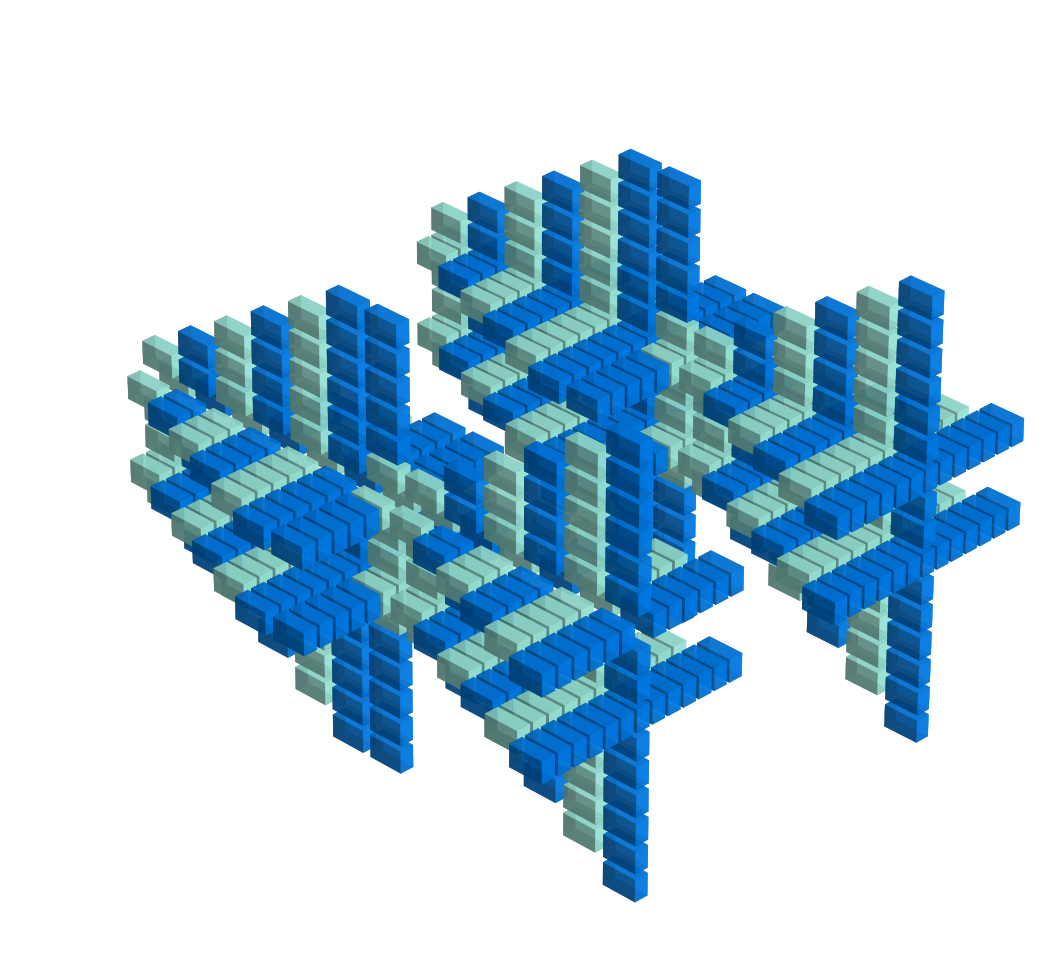
\includegraphics[width=14cm]{src/presets/pattern9-45.png}%           
  \end{adjustbox}                                                        
\caption{Evolution of Preset 9.}                                           
\end{figure}                                                               
\clearpage                                                                 
                                                                           
\begin{lstlisting}[basicstyle=\ttfamily\scriptsize,caption=Data structure for Preset 9.]
preset9
  ; unusedPresetByte: Unused Byte
  .BYTE $00
  ; smoothingDelay: 'Because of the time taken to draw larger patterns speed
  ; increase/decrease is not linear. You can adjust the 'compensating delay'
  ; which often smooths out jerky patterns. Can be used just for special FX),
  ; though. Suck it and see.'
  .BYTE $11
  ; cursorSpeed: 'Gives you a slow or fast little cursor, according to setting.'
  .BYTE $01
  ; bufferLength: 'Larger patterns flow more smoothly with a shorter
  ; Buffer Length - not so many positions are retained so less plotting to do.
  ; Small patterns with a long Buffer Length are good for 'steamer' effects.
  ; N.B. Cannot be adjusted whilst patterns are actually onscreen.'
  .BYTE $0D
  ; pulseSpeed: 'Usually if you hold down the button you get a continuous
  ; stream. Setting the Pulse Speed allows you to generate a pulsed stream, as
  ; if you were rapidly pressing and releasing the FIRE button.'
  .BYTE $07
  ; indexForColorBarDisplay: 'The initial index for the color displayed
  ; in the color bar when adjusting the colors for each step.'
  .BYTE $01
  ; lineWidth: 'Sets the width of the lines produced in Line Mode.'
  .BYTE $07
  ; sequencerSpeed: 'Controls the rate at which sequencer feeds in its data. '
  .BYTE $0C
  ; pulseWidth: 'Sets the length of the pulses in a pulsed stream output.
  ; Don't worry about what that means - just get in there and mess with it.'
  .BYTE $01
  ; baseLevel: 'Controls how many 'levels' of pattern are plotted.'
  .BYTE $07
  ; presetColorValuesArray: 'Allows you to set the colour for each of the
  ; seven pattern steps. Set up the colour you want, press RETURN, and the
  ; command offers the next colour along, up to no. 7, then ends. Cannot be
  ; adjusted while patterns being generated.'
  .BYTE BLACK,BLUE,CYAN,BLUE,CYAN,BLUE,CYAN,BLUE
  ; trackingActivated: 'Controls whether logic-seeking is used in the
  ; buffer or not. The upshot of this for you is a slightly different feel -
  ; continuous but fragmented when ON, or together-ish bursts when OFF. Try it.'
  .BYTE $FF
  ; lineModeActivated: 'A bit like drawing with the Aurora Borealis'
  .BYTE $00
  ; presetIndex: 'This calls in one of the 16 presets, stored Lightsynth
  ; parameters which give different effects. Try them all out io see some uf
  ; the multitude of effects which you cai achieve using the system. Some are
  ; fast, some slow, some pulse, others swirl. Play with them all, try them to
  ; different music.'
  .BYTE $07
  ; currentPatternElement: 'Initial pattern used by this preset.'
  .BYTE $07
  ; currentSymmetrySetting: 'Current symmetry setting.'
  ; Possible values are 0 - 4:
  ; 'NO SYMMETRY     '
  ; 'Y-AXIS SYMMETRY '
  ; 'X-Y SYMMETRY    '
  ; 'X-AXIS SYMMETRY '
  ; 'QUAD SYMMETRY   '
  .BYTE $04
  ; Unused Data.
  .BYTE $FF,$00,$FF,$FF,$00,$FF,$00,$FF,$00
\end{lstlisting}


\clearpage                                                                 
\begin{figure}[H]                                                          
  \centering                                                             
  \begin{adjustbox}{width=14cm,center}                                   
  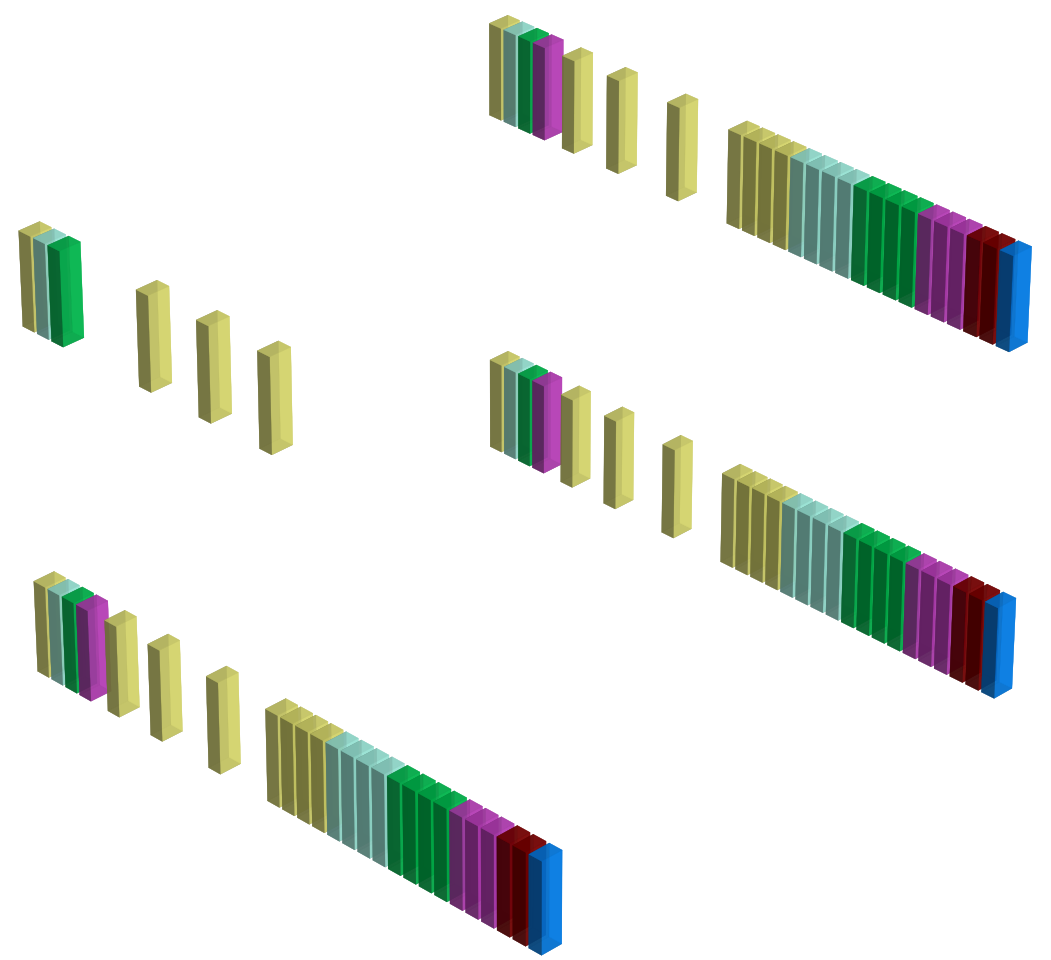
\includegraphics[width=14cm]{src/presets/pattern10-45.png}%           
  \end{adjustbox}                                                        
\caption{Evolution of Preset 10.}                                           
\end{figure}                                                               
\clearpage                                                                 
                                                                           
\begin{lstlisting}[basicstyle=\ttfamily\scriptsize,caption=Data structure for Preset 10.]
preset10
  ; unusedPresetByte: Unused Byte
  .BYTE $00
  ; smoothingDelay: 'Because of the time taken to draw larger patterns speed
  ; increase/decrease is not linear. You can adjust the 'compensating delay'
  ; which often smooths out jerky patterns. Can be used just for special FX),
  ; though. Suck it and see.'
  .BYTE $01
  ; cursorSpeed: 'Gives you a slow or fast little cursor, according to setting.'
  .BYTE $02
  ; bufferLength: 'Larger patterns flow more smoothly with a shorter
  ; Buffer Length - not so many positions are retained so less plotting to do.
  ; Small patterns with a long Buffer Length are good for 'steamer' effects.
  ; N.B. Cannot be adjusted whilst patterns are actually onscreen.'
  .BYTE $1F
  ; pulseSpeed: 'Usually if you hold down the button you get a continuous
  ; stream. Setting the Pulse Speed allows you to generate a pulsed stream, as
  ; if you were rapidly pressing and releasing the FIRE button.'
  .BYTE $02
  ; indexForColorBarDisplay: 'The initial index for the color displayed
  ; in the color bar when adjusting the colors for each step.'
  .BYTE $09
  ; lineWidth: 'Sets the width of the lines produced in Line Mode.'
  .BYTE $04
  ; sequencerSpeed: 'Controls the rate at which sequencer feeds in its data. '
  .BYTE $08
  ; pulseWidth: 'Sets the length of the pulses in a pulsed stream output.
  ; Don't worry about what that means - just get in there and mess with it.'
  .BYTE $01
  ; baseLevel: 'Controls how many 'levels' of pattern are plotted.'
  .BYTE $07
  ; presetColorValuesArray: 'Allows you to set the colour for each of the
  ; seven pattern steps. Set up the colour you want, press RETURN, and the
  ; command offers the next colour along, up to no. 7, then ends. Cannot be
  ; adjusted while patterns being generated.'
  .BYTE BLACK,BLUE,RED,RED,PURPLE,LTRED,ORANGE,BROWN
  ; trackingActivated: 'Controls whether logic-seeking is used in the
  ; buffer or not. The upshot of this for you is a slightly different feel -
  ; continuous but fragmented when ON, or together-ish bursts when OFF. Try it.'
  .BYTE $FF
  ; lineModeActivated: 'A bit like drawing with the Aurora Borealis'
  .BYTE $01
  ; presetIndex: 'This calls in one of the 16 presets, stored Lightsynth
  ; parameters which give different effects. Try them all out io see some uf
  ; the multitude of effects which you cai achieve using the system. Some are
  ; fast, some slow, some pulse, others swirl. Play with them all, try them to
  ; different music.'
  .BYTE $00
  ; currentPatternElement: 'Initial pattern used by this preset.'
  .BYTE $00
  ; currentSymmetrySetting: 'Current symmetry setting.'
  ; Possible values are 0 - 4:
  ; 'NO SYMMETRY     '
  ; 'Y-AXIS SYMMETRY '
  ; 'X-Y SYMMETRY    '
  ; 'X-AXIS SYMMETRY '
  ; 'QUAD SYMMETRY   '
  .BYTE $04
  ; Unused Data.
  .BYTE $FF,$00,$FF,$FF,$00,$FF,$00,$FF,$00
\end{lstlisting}


\clearpage                                                                 
\begin{figure}[H]                                                          
  \centering                                                             
  \begin{adjustbox}{width=14cm,center}                                   
  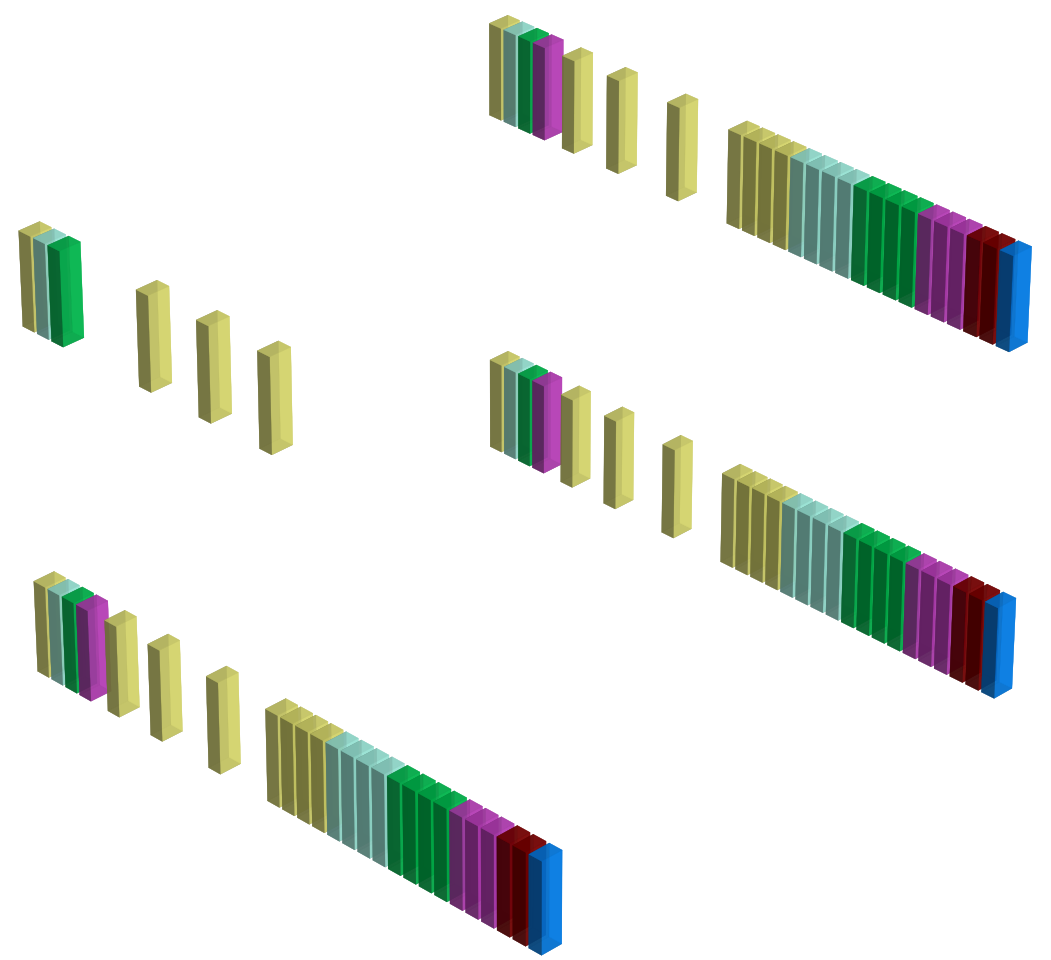
\includegraphics[width=14cm]{src/presets/pattern10-45.png}%           
  \end{adjustbox}                                                        
\caption{Evolution of Preset 11.}                                           
\end{figure}                                                               
\clearpage                                                                 
                                                                           
\begin{lstlisting}[basicstyle=\ttfamily\scriptsize,caption=Data structure for Preset 11.]
preset11
  ; unusedPresetByte: Unused Byte
  .BYTE $00
  ; smoothingDelay: 'Because of the time taken to draw larger patterns speed
  ; increase/decrease is not linear. You can adjust the 'compensating delay'
  ; which often smooths out jerky patterns. Can be used just for special FX),
  ; though. Suck it and see.'
  .BYTE $01
  ; cursorSpeed: 'Gives you a slow or fast little cursor, according to setting.'
  .BYTE $01
  ; bufferLength: 'Larger patterns flow more smoothly with a shorter
  ; Buffer Length - not so many positions are retained so less plotting to do.
  ; Small patterns with a long Buffer Length are good for 'steamer' effects.
  ; N.B. Cannot be adjusted whilst patterns are actually onscreen.'
  .BYTE $13
  ; pulseSpeed: 'Usually if you hold down the button you get a continuous
  ; stream. Setting the Pulse Speed allows you to generate a pulsed stream, as
  ; if you were rapidly pressing and releasing the FIRE button.'
  .BYTE $06
  ; indexForColorBarDisplay: 'The initial index for the color displayed
  ; in the color bar when adjusting the colors for each step.'
  .BYTE $01
  ; lineWidth: 'Sets the width of the lines produced in Line Mode.'
  .BYTE $07
  ; sequencerSpeed: 'Controls the rate at which sequencer feeds in its data. '
  .BYTE $08
  ; pulseWidth: 'Sets the length of the pulses in a pulsed stream output.
  ; Don't worry about what that means - just get in there and mess with it.'
  .BYTE $05
  ; baseLevel: 'Controls how many 'levels' of pattern are plotted.'
  .BYTE $07
  ; presetColorValuesArray: 'Allows you to set the colour for each of the
  ; seven pattern steps. Set up the colour you want, press RETURN, and the
  ; command offers the next colour along, up to no. 7, then ends. Cannot be
  ; adjusted while patterns being generated.'
  .BYTE BLACK,BLUE,RED,PURPLE,GREEN,CYAN,YELLOW,WHITE
  ; trackingActivated: 'Controls whether logic-seeking is used in the
  ; buffer or not. The upshot of this for you is a slightly different feel -
  ; continuous but fragmented when ON, or together-ish bursts when OFF. Try it.'
  .BYTE $FF
  ; lineModeActivated: 'A bit like drawing with the Aurora Borealis'
  .BYTE $00
  ; presetIndex: 'This calls in one of the 16 presets, stored Lightsynth
  ; parameters which give different effects. Try them all out io see some uf
  ; the multitude of effects which you cai achieve using the system. Some are
  ; fast, some slow, some pulse, others swirl. Play with them all, try them to
  ; different music.'
  .BYTE $0F
  ; currentPatternElement: 'Initial pattern used by this preset.'
  .BYTE $0F
  ; currentSymmetrySetting: 'Current symmetry setting.'
  ; Possible values are 0 - 4:
  ; 'NO SYMMETRY     '
  ; 'Y-AXIS SYMMETRY '
  ; 'X-Y SYMMETRY    '
  ; 'X-AXIS SYMMETRY '
  ; 'QUAD SYMMETRY   '
  .BYTE $04
  ; Unused Data.
  .BYTE $FF,$00,$FF,$FF,$00,$FF,$00,$EA,$10
\end{lstlisting}


\clearpage                                                                 
\begin{figure}[H]                                                          
  \centering                                                             
  \begin{adjustbox}{width=14cm,center}                                   
  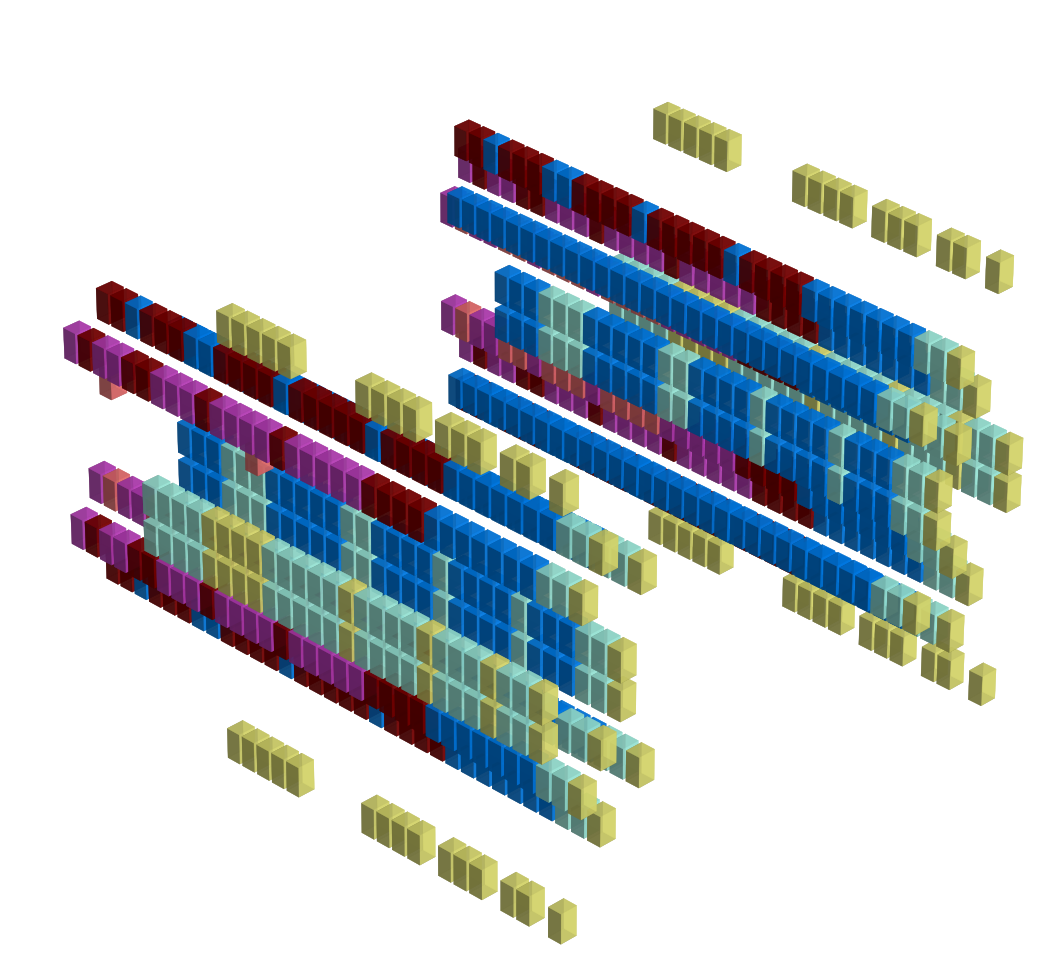
\includegraphics[width=14cm]{src/presets/pattern12-45.png}%           
  \end{adjustbox}                                                        
\caption{Evolution of Preset 12.}                                           
\end{figure}                                                               
\clearpage                                                                 
                                                                           
\begin{lstlisting}[basicstyle=\ttfamily\scriptsize,caption=Data structure for Preset 12.]
preset12
  ; unusedPresetByte: Unused Byte
  .BYTE $00
  ; smoothingDelay: 'Because of the time taken to draw larger patterns speed
  ; increase/decrease is not linear. You can adjust the 'compensating delay'
  ; which often smooths out jerky patterns. Can be used just for special FX),
  ; though. Suck it and see.'
  .BYTE $0C
  ; cursorSpeed: 'Gives you a slow or fast little cursor, according to setting.'
  .BYTE $02
  ; bufferLength: 'Larger patterns flow more smoothly with a shorter
  ; Buffer Length - not so many positions are retained so less plotting to do.
  ; Small patterns with a long Buffer Length are good for 'steamer' effects.
  ; N.B. Cannot be adjusted whilst patterns are actually onscreen.'
  .BYTE $28
  ; pulseSpeed: 'Usually if you hold down the button you get a continuous
  ; stream. Setting the Pulse Speed allows you to generate a pulsed stream, as
  ; if you were rapidly pressing and releasing the FIRE button.'
  .BYTE $01
  ; indexForColorBarDisplay: 'The initial index for the color displayed
  ; in the color bar when adjusting the colors for each step.'
  .BYTE $02
  ; lineWidth: 'Sets the width of the lines produced in Line Mode.'
  .BYTE $07
  ; sequencerSpeed: 'Controls the rate at which sequencer feeds in its data. '
  .BYTE $09
  ; pulseWidth: 'Sets the length of the pulses in a pulsed stream output.
  ; Don't worry about what that means - just get in there and mess with it.'
  .BYTE $01
  ; baseLevel: 'Controls how many 'levels' of pattern are plotted.'
  .BYTE $07
  ; presetColorValuesArray: 'Allows you to set the colour for each of the
  ; seven pattern steps. Set up the colour you want, press RETURN, and the
  ; command offers the next colour along, up to no. 7, then ends. Cannot be
  ; adjusted while patterns being generated.'
  .BYTE BLACK,BLUE,LTBLUE,CYAN,LTGREEN,YELLOW,PURPLE,RED
  ; trackingActivated: 'Controls whether logic-seeking is used in the
  ; buffer or not. The upshot of this for you is a slightly different feel -
  ; continuous but fragmented when ON, or together-ish bursts when OFF. Try it.'
  .BYTE $00
  ; lineModeActivated: 'A bit like drawing with the Aurora Borealis'
  .BYTE $00
  ; presetIndex: 'This calls in one of the 16 presets, stored Lightsynth
  ; parameters which give different effects. Try them all out io see some uf
  ; the multitude of effects which you cai achieve using the system. Some are
  ; fast, some slow, some pulse, others swirl. Play with them all, try them to
  ; different music.'
  .BYTE $0A
  ; currentPatternElement: 'Initial pattern used by this preset.'
  .BYTE $0A
  ; currentSymmetrySetting: 'Current symmetry setting.'
  ; Possible values are 0 - 4:
  ; 'NO SYMMETRY     '
  ; 'Y-AXIS SYMMETRY '
  ; 'X-Y SYMMETRY    '
  ; 'X-AXIS SYMMETRY '
  ; 'QUAD SYMMETRY   '
  .BYTE $01
  ; Unused Data.
  .BYTE $00,$FF,$00,$00,$FF,$00,$FF,$00,$FF
\end{lstlisting}


\clearpage                                                                 
\begin{figure}[H]                                                          
  \centering                                                             
  \begin{adjustbox}{width=14cm,center}                                   
  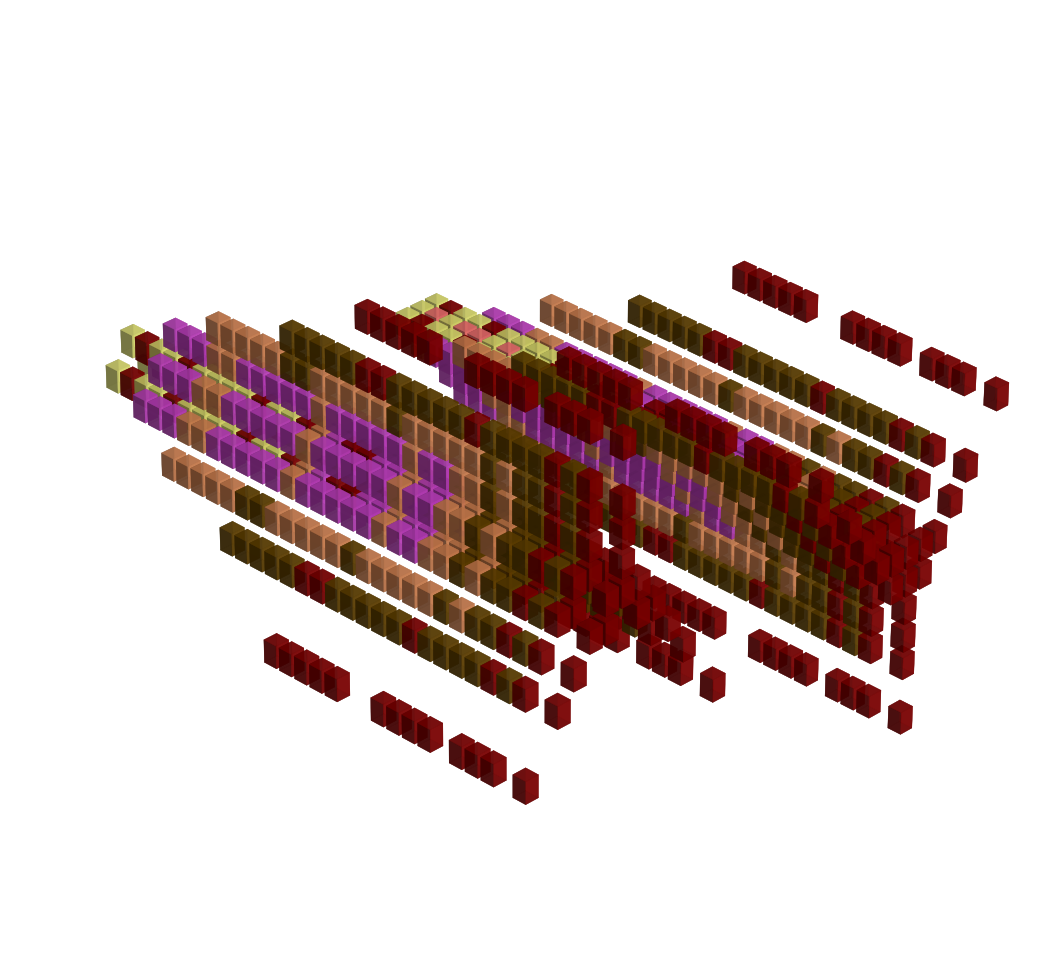
\includegraphics[width=14cm]{src/presets/pattern13-45.png}%           
  \end{adjustbox}                                                        
\caption{Evolution of Preset 13.}                                           
\end{figure}                                                               
\clearpage                                                                 
                                                                           
\begin{lstlisting}[basicstyle=\ttfamily\scriptsize,caption=Data structure for Preset 13.]
preset13
  ; unusedPresetByte: Unused Byte
  .BYTE $00
  ; smoothingDelay: 'Because of the time taken to draw larger patterns speed
  ; increase/decrease is not linear. You can adjust the 'compensating delay'
  ; which often smooths out jerky patterns. Can be used just for special FX),
  ; though. Suck it and see.'
  .BYTE $0B
  ; cursorSpeed: 'Gives you a slow or fast little cursor, according to setting.'
  .BYTE $01
  ; bufferLength: 'Larger patterns flow more smoothly with a shorter
  ; Buffer Length - not so many positions are retained so less plotting to do.
  ; Small patterns with a long Buffer Length are good for 'steamer' effects.
  ; N.B. Cannot be adjusted whilst patterns are actually onscreen.'
  .BYTE $1C
  ; pulseSpeed: 'Usually if you hold down the button you get a continuous
  ; stream. Setting the Pulse Speed allows you to generate a pulsed stream, as
  ; if you were rapidly pressing and releasing the FIRE button.'
  .BYTE $02
  ; indexForColorBarDisplay: 'The initial index for the color displayed
  ; in the color bar when adjusting the colors for each step.'
  .BYTE $0A
  ; lineWidth: 'Sets the width of the lines produced in Line Mode.'
  .BYTE $07
  ; sequencerSpeed: 'Controls the rate at which sequencer feeds in its data. '
  .BYTE $09
  ; pulseWidth: 'Sets the length of the pulses in a pulsed stream output.
  ; Don't worry about what that means - just get in there and mess with it.'
  .BYTE $01
  ; baseLevel: 'Controls how many 'levels' of pattern are plotted.'
  .BYTE $07
  ; presetColorValuesArray: 'Allows you to set the colour for each of the
  ; seven pattern steps. Set up the colour you want, press RETURN, and the
  ; command offers the next colour along, up to no. 7, then ends. Cannot be
  ; adjusted while patterns being generated.'
  .BYTE BLACK,YELLOW,CYAN,LTBLUE,BLUE,RED,PURPLE,LTRED
  ; trackingActivated: 'Controls whether logic-seeking is used in the
  ; buffer or not. The upshot of this for you is a slightly different feel -
  ; continuous but fragmented when ON, or together-ish bursts when OFF. Try it.'
  .BYTE $00
  ; lineModeActivated: 'A bit like drawing with the Aurora Borealis'
  .BYTE $00
  ; presetIndex: 'This calls in one of the 16 presets, stored Lightsynth
  ; parameters which give different effects. Try them all out io see some uf
  ; the multitude of effects which you cai achieve using the system. Some are
  ; fast, some slow, some pulse, others swirl. Play with them all, try them to
  ; different music.'
  .BYTE $03
  ; currentPatternElement: 'Initial pattern used by this preset.'
  .BYTE $03
  ; currentSymmetrySetting: 'Current symmetry setting.'
  ; Possible values are 0 - 4:
  ; 'NO SYMMETRY     '
  ; 'Y-AXIS SYMMETRY '
  ; 'X-Y SYMMETRY    '
  ; 'X-AXIS SYMMETRY '
  ; 'QUAD SYMMETRY   '
  .BYTE $04
  ; Unused Data.
  .BYTE $00,$FF,$00,$00,$FF,$00,$FF,$00,$FF
\end{lstlisting}


\clearpage                                                                 
\begin{figure}[H]                                                          
  \centering                                                             
  \begin{adjustbox}{width=14cm,center}                                   
  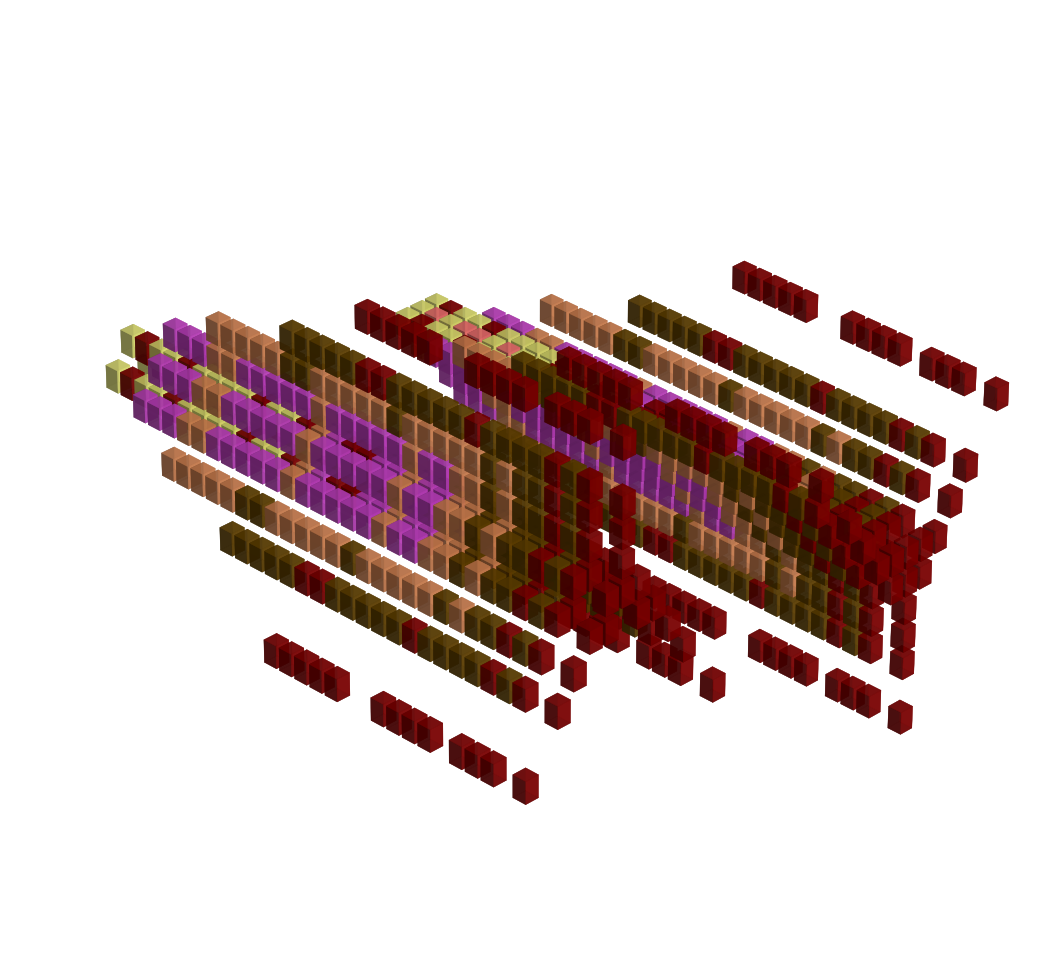
\includegraphics[width=14cm]{src/presets/pattern14-45.png}%           
  \end{adjustbox}                                                        
\caption{Evolution of Preset 14.}                                           
\end{figure}                                                               
\clearpage                                                                 
                                                                           
\begin{lstlisting}[basicstyle=\ttfamily\scriptsize,caption=Data structure for Preset 14.]
preset14
  ; unusedPresetByte: Unused Byte
  .BYTE $00
  ; smoothingDelay: 'Because of the time taken to draw larger patterns speed
  ; increase/decrease is not linear. You can adjust the 'compensating delay'
  ; which often smooths out jerky patterns. Can be used just for special FX),
  ; though. Suck it and see.'
  .BYTE $0C
  ; cursorSpeed: 'Gives you a slow or fast little cursor, according to setting.'
  .BYTE $02
  ; bufferLength: 'Larger patterns flow more smoothly with a shorter
  ; Buffer Length - not so many positions are retained so less plotting to do.
  ; Small patterns with a long Buffer Length are good for 'steamer' effects.
  ; N.B. Cannot be adjusted whilst patterns are actually onscreen.'
  .BYTE $2B
  ; pulseSpeed: 'Usually if you hold down the button you get a continuous
  ; stream. Setting the Pulse Speed allows you to generate a pulsed stream, as
  ; if you were rapidly pressing and releasing the FIRE button.'
  .BYTE $01
  ; indexForColorBarDisplay: 'The initial index for the color displayed
  ; in the color bar when adjusting the colors for each step.'
  .BYTE $0A
  ; lineWidth: 'Sets the width of the lines produced in Line Mode.'
  .BYTE $07
  ; sequencerSpeed: 'Controls the rate at which sequencer feeds in its data. '
  .BYTE $08
  ; pulseWidth: 'Sets the length of the pulses in a pulsed stream output.
  ; Don't worry about what that means - just get in there and mess with it.'
  .BYTE $01
  ; baseLevel: 'Controls how many 'levels' of pattern are plotted.'
  .BYTE $07
  ; presetColorValuesArray: 'Allows you to set the colour for each of the
  ; seven pattern steps. Set up the colour you want, press RETURN, and the
  ; command offers the next colour along, up to no. 7, then ends. Cannot be
  ; adjusted while patterns being generated.'
  .BYTE BLACK,RED,BROWN,ORANGE,PURPLE,RED,YELLOW,LTRED
  ; trackingActivated: 'Controls whether logic-seeking is used in the
  ; buffer or not. The upshot of this for you is a slightly different feel -
  ; continuous but fragmented when ON, or together-ish bursts when OFF. Try it.'
  .BYTE $FF
  ; lineModeActivated: 'A bit like drawing with the Aurora Borealis'
  .BYTE $00
  ; presetIndex: 'This calls in one of the 16 presets, stored Lightsynth
  ; parameters which give different effects. Try them all out io see some uf
  ; the multitude of effects which you cai achieve using the system. Some are
  ; fast, some slow, some pulse, others swirl. Play with them all, try them to
  ; different music.'
  .BYTE $04
  ; currentPatternElement: 'Initial pattern used by this preset.'
  .BYTE $04
  ; currentSymmetrySetting: 'Current symmetry setting.'
  ; Possible values are 0 - 4:
  ; 'NO SYMMETRY     '
  ; 'Y-AXIS SYMMETRY '
  ; 'X-Y SYMMETRY    '
  ; 'X-AXIS SYMMETRY '
  ; 'QUAD SYMMETRY   '
  .BYTE $02
  ; Unused Data.
  .BYTE $00,$FF,$00,$00,$FF,$00,$FF,$00,$FF
\end{lstlisting}


\clearpage                                                                 
\begin{figure}[H]                                                          
  \centering                                                             
  \begin{adjustbox}{width=14cm,center}                                   
  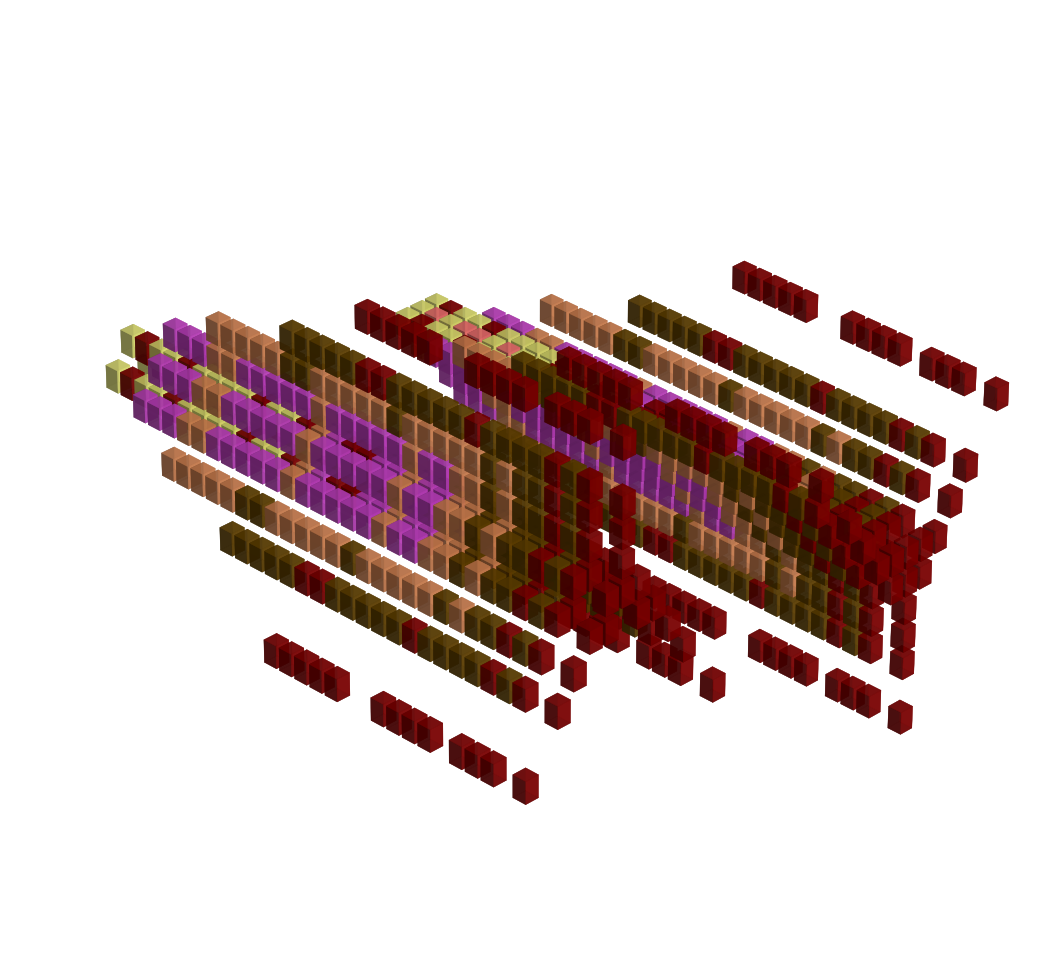
\includegraphics[width=14cm]{src/presets/pattern14-45.png}%           
  \end{adjustbox}                                                        
\caption{Evolution of Preset 15.}                                           
\end{figure}                                                               
\clearpage                                                                 
                                                                           
\begin{lstlisting}[basicstyle=\ttfamily\scriptsize,caption=Data structure for Preset 15.]
preset15
  ; unusedPresetByte: Unused Byte
  .BYTE $00
  ; smoothingDelay: 'Because of the time taken to draw larger patterns speed
  ; increase/decrease is not linear. You can adjust the 'compensating delay'
  ; which often smooths out jerky patterns. Can be used just for special FX),
  ; though. Suck it and see.'
  .BYTE $03
  ; cursorSpeed: 'Gives you a slow or fast little cursor, according to setting.'
  .BYTE $01
  ; bufferLength: 'Larger patterns flow more smoothly with a shorter
  ; Buffer Length - not so many positions are retained so less plotting to do.
  ; Small patterns with a long Buffer Length are good for 'steamer' effects.
  ; N.B. Cannot be adjusted whilst patterns are actually onscreen.'
  .BYTE $1F
  ; pulseSpeed: 'Usually if you hold down the button you get a continuous
  ; stream. Setting the Pulse Speed allows you to generate a pulsed stream, as
  ; if you were rapidly pressing and releasing the FIRE button.'
  .BYTE $06
  ; indexForColorBarDisplay: 'The initial index for the color displayed
  ; in the color bar when adjusting the colors for each step.'
  .BYTE $01
  ; lineWidth: 'Sets the width of the lines produced in Line Mode.'
  .BYTE $07
  ; sequencerSpeed: 'Controls the rate at which sequencer feeds in its data. '
  .BYTE $00
  ; pulseWidth: 'Sets the length of the pulses in a pulsed stream output.
  ; Don't worry about what that means - just get in there and mess with it.'
  .BYTE $01
  ; baseLevel: 'Controls how many 'levels' of pattern are plotted.'
  .BYTE $07
  ; presetColorValuesArray: 'Allows you to set the colour for each of the
  ; seven pattern steps. Set up the colour you want, press RETURN, and the
  ; command offers the next colour along, up to no. 7, then ends. Cannot be
  ; adjusted while patterns being generated.'
  .BYTE BLACK,BLUE,RED,PURPLE,GREEN,CYAN,YELLOW,WHITE
  ; trackingActivated: 'Controls whether logic-seeking is used in the
  ; buffer or not. The upshot of this for you is a slightly different feel -
  ; continuous but fragmented when ON, or together-ish bursts when OFF. Try it.'
  .BYTE $FF
  ; lineModeActivated: 'A bit like drawing with the Aurora Borealis'
  .BYTE $00
  ; presetIndex: 'This calls in one of the 16 presets, stored Lightsynth
  ; parameters which give different effects. Try them all out io see some uf
  ; the multitude of effects which you cai achieve using the system. Some are
  ; fast, some slow, some pulse, others swirl. Play with them all, try them to
  ; different music.'
  .BYTE $04
  ; currentPatternElement: 'Initial pattern used by this preset.'
  .BYTE $04
  ; currentSymmetrySetting: 'Current symmetry setting.'
  ; Possible values are 0 - 4:
  ; 'NO SYMMETRY     '
  ; 'Y-AXIS SYMMETRY '
  ; 'X-Y SYMMETRY    '
  ; 'X-AXIS SYMMETRY '
  ; 'QUAD SYMMETRY   '
  .BYTE $04
  ; Unused Data.
  .BYTE $00,$FF,$00,$00,$FF,$00,$FF,$15,$EF
\end{lstlisting}

